\documentclass[
    letterpaper, 
    man,   
    spanish,
    12pt,
    donotrepeattitle,
    floatsintext,
    hidelinks % Opción para hyperref pasada a la clase
]{apa7}

% --- Codificación y Lenguaje ---
\usepackage[utf8]{inputenc} 
\usepackage{newunicodechar}
\usepackage[spanish]{babel} 
\selectlanguage{spanish}   
\usepackage{csquotes}       

% --- Definición de caracteres Unicode problemáticos ---
\newunicodechar{́}{'}  % U+0301 COMBINING ACUTE ACCENT
\newunicodechar{—}{---}  % U+2014 EM DASH
\newunicodechar{ć}{c'}  % U+0107 LATIN SMALL LETTER C WITH ACUTE
\newunicodechar{ı}{i}  % U+0131 LATIN SMALL LETTER DOTLESS I

% --- Bibliografía con biblatex-apa ---
\usepackage[
    style=apa,            
    backend=biber,        
    sortcites=true,       
    sorting=nyt,          
    hyperref=true,
    backref=false         
]{biblatex}
\DeclareLanguageMapping{spanish}{spanish-apa}
\addbibresource{bibliography.bib} 

% --- Paquetes para Gráficos y Tablas ---
\usepackage{graphicx}     
\usepackage{booktabs}     
\usepackage{adjustbox}    
\usepackage{multirow}     
\usepackage{array}
% \usepackage{epstopdf}    
% \usepackage{float}       

% --- COMANDOS PERSONALIZADOS
 \newcommand{\myparagraph}[1]{\paragraph{#1}\mbox{}\\} % Esto 
% --- Definición de comandos de tamaño de fuente ---
\renewcommand{\large}{\fontsize{14.4}{18}\selectfont}

% --- Información del Documento (Ejemplo) ---

\title{Prototipo de sistema descentralizado para la gestión y verificación de evidencias digitales en fotocomparendos aplicando Blockchain e IPFS }
\shorttitle{Gestion de Comparendos}
\author{Laura Catalina Preciado Ballen \\Cristian Stiven Guzman Tovar}
\affiliation{Universidad Distrital Francisco José de Caldas}
\course{Proyecto de grado para optar al título de: \\Ingeniero (a) de Sistemas}
\professor{Julio Baron Velandia}
\duedate{\today}
\abstract{Este trabajo propone el diseño e implementación de un prototipo basado en Blockchain para la gestión de fotocomparendos en Bogotá, con el objetivo de garantizar la transparencia del proceso. Se utilizarán contratos inteligentes para registrar cada infracción, permitiendo que cualquier actor autorizado pueda verificar su autenticidad sin necesidad de intermediarios. Mediante pruebas y simulaciones, se evaluará la viabilidad del sistema, demostrando cómo esta tecnología puede fortalecer la confianza en los procesos de control de tránsito y mejorar la eficiencia en la gestión de sanciones. }
\keywords{Fotocomparendos, Gestion de datos, Blockchain, ingeniería web}

\begin{document}
% \maketitle
%Preguntar cual dejar?
\begin{titlepage}
    \begin{center}
        \vspace*{0.5cm}
            
        \Large
        \textbf{Prototipo de sistema descentralizado para la gestión y verificación de evidencias digitales en fotocomparendos aplicando Blockchain e IPFS}
            
        
        \vspace{2.5cm}
            
        \normalsize
        \textbf{Laura Catalina Preciado Ballen}\\
        \textbf{Cristian Stiven Guzman Tovar}
            
        \vfill
            
        Proyecto de Monografía para Optar por el Título de\\
        Ingeniero(a) de Sistemas
            
        \vspace{0.8cm}
            
        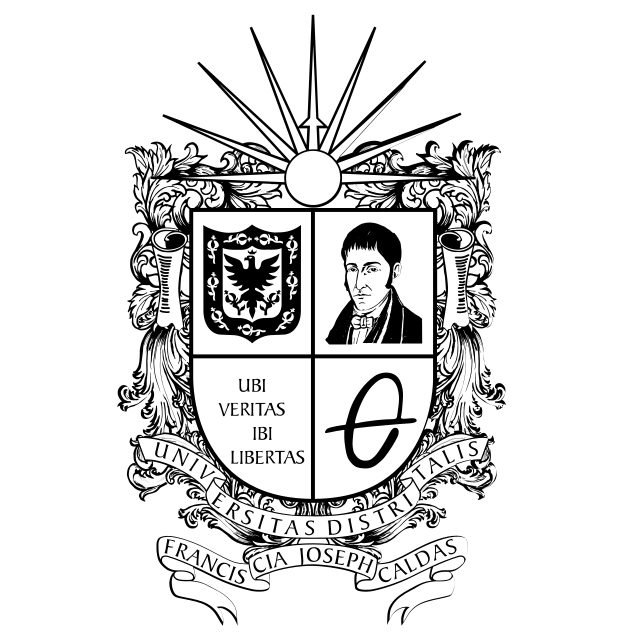
\includegraphics[width=0.2\textwidth]{Images/Escudo_UD}
            
        \large
        Universidad Distrital Francisco José De Caldas\\
        Facultad de Ingeniería\\
        Colombia, Bogotá D.C.\\
        Julio de 2025\\

        
            
    \end{center}
\end{titlepage}

\raggedbottom 

\pagenumbering{roman}
    % Contenido
\renewcommand\contentsname{\textbf{Índice}}
\tableofcontents
\setcounter{tocdepth}{2}
\newpage
    % Fíguras
\renewcommand{\listfigurename}{\textbf{Índice de figuras}}
\listoffigures
\newpage
    % Tablas
\renewcommand{\listtablename}{\textbf{Índice de tablas}}
\listoftables
\newpage

% Cuerpo
\pagenumbering{arabic}

\section{\large Introducción}
En Colombia, la gestión de fotocomparendos ha sido objeto de controversia debido a fallas en la transparencia y posibles manipulaciones en el proceso de registro y validación de infracciones. La falta de un sistema confiable ha generado desconfianza entre los ciudadanos, lo que evidencia la necesidad de una solución que garantice la integridad, inmutabilidad y verificabilidad de la información.

La tecnología Blockchain ha demostrado ser una alternativa eficaz para el almacenamiento seguro y descentralizado de datos, asegurando que una vez registrados, estos no puedan ser alterados sin dejar rastro. A través de contratos inteligentes, es posible automatizar la validación y el procesamiento de fotocomparendos, reduciendo la intervención humana y minimizando el riesgo de corrupción o errores administrativos.

Este trabajo propone el diseño e implementación de un prototipo basado en Blockchain para la gestión de fotocomparendos en Bogotá, con el objetivo de garantizar la transparencia del proceso. Se utilizarán contratos inteligentes para registrar cada infracción, permitiendo que cualquier actor autorizado pueda verificar su autenticidad sin necesidad de intermediarios. Mediante pruebas y simulaciones, se evaluará la viabilidad del sistema, demostrando cómo esta tecnología puede fortalecer la confianza en los procesos de control de tránsito y mejorar la eficiencia en la gestión de sanciones.

\subsection{Formulación del problema}
El sistema actual de gestión de fotocomparendos en Bogotá, enfrenta serias limitaciones en términos de transparencia, seguridad e integridad de la información, lo que genera desconfianza por parte de la ciudadanía y dificultades administrativas en su gestión. Según el Observatorio de Movilidad de Bogotá, entre enero de 2018 y agosto de 2024 se emitieron 5.575.982 comparendos, de los cuales el 48,91 \% fueron generados mediante dispositivos electrónicos de asistencia policial \parencite{ObservatorioComparendos2025}

\begin{adjustbox}{
    center,
    caption=[{Tomado del Observatorio de Movilidad}]{\centering Tomado del Observatorio de Movilidad},
    label={EstadisticasComparendos},
    nofloat=figure, vspace={7px}}

    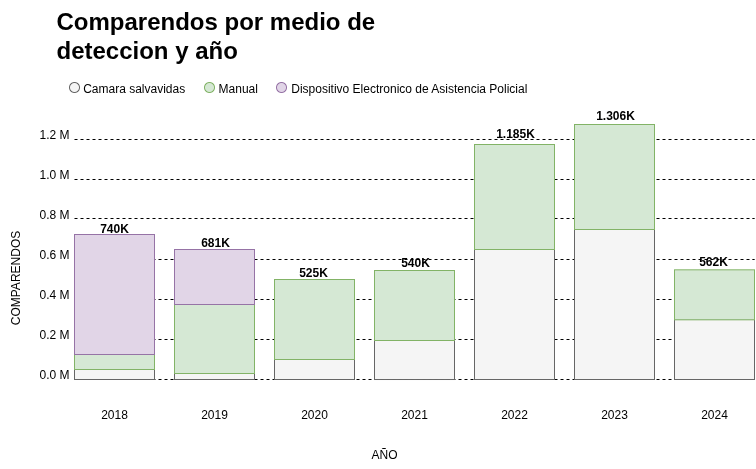
\includegraphics[width=0.8\textwidth]{Images/numComparendos.png}
\end{adjustbox}

Estas cifras reflejan el papel protagónico que tienen las fotomultas en la regulación del tránsito en la ciudad, pero también resaltan la necesidad urgente de fortalecer los mecanismos de manejo, almacenamiento y verificación de evidencias.  

La ausencia de un sistema confiable y auditable que permita garantizar la inmutabilidad de los registros, así como la trazabilidad de las evidencias, ha generado un entorno donde se cuestiona la validez de las sanciones, se incrementan las quejas ciudadanas y se limita la eficiencia operativa de las entidades encargadas del control de tránsito. En este contexto, surge la necesidad de explorar tecnologías emergentes, como Blockchain e IPFS, que podrían ofrecer una solución más segura, descentralizada y transparente para la gestión de estos procesos. 

\subsection{Objetivos}
\paragraph{Objetivo General}
Desarrollar un prototipo funcional que utilice tecnología Blockchain e IPFS (InterPlanetary File System)  para la gestión segura, transparente y descentralizada de evidencias digitales asociadas a foto comparendos, con el fin de mejorar la confiabilidad y eficiencia del proceso en el contexto de la ciudad de Bogotá. 

\paragraph{Objetivos específicos}
\begin{itemize}
    \item Analizar el proceso actual de gestión de fotocomparendos en Bogotá, mediante la revisión de normativa, flujos de trabajo documentados, para identificar las vulnerabilidades y los requisitos funcionales y no funcionales (seguridad, rendimiento y auditabilidad) que el prototipo Blockchain debe satisfacer, resultando en una lista de requerimientos específicos para la nueva solución.
    \item Construir el prototipo del sistema de gestión de foto comparendos, implementando la arquitectura propuesta (IPFS para almacenamiento de imágenes y Hyperledger Fabric para el registro de transacciones), asegurando que cada transacción contenga el hash único de IPFS y los metadatos esenciales del comparendo (fecha, hora, lugar, placa, tipo de infracción), y desarrollando una interfaz básica que permita la carga de la evidencia y la consulta/verificación de los registros en la blockchain y la imagen en IPFS, con el fin de materializar técnicamente la solución propuesta basada en los requisitos identificados en el objetivo anterior.
    \item Evaluar la efectividad y viabilidad del prototipo desarrollado, mediante la ejecución de un plan de pruebas funcionales (verificar la correcta carga a IPFS, el registro inmutable en el ledger, la consistencia de datos, la capacidad de verificación) y pruebas de rendimiento básicas (medir tiempos de registro y consulta) en un entorno de simulación controlado, para validar que el prototipo cumple con los requisitos clave de inmutabilidad, transparencia y seguridad.
\end{itemize}

\newpage
\section{\large Justificación}

La gestión actual de los fotocomparendos en Bogotá, articulada principalmente a través del sistema FENIX —desarrollado por la Oficina de Tecnologías de la Información y las Comunicaciones con una inversión de \$3.800 millones de pesos colombianos— presenta limitaciones críticas que afectan la transparencia, seguridad y confianza pública en el proceso sancionatorio vial \parencite{resolucionFenix}.

Uno de los principales desafíos es el riesgo constante de corrupción. Existen evidencias documentadas de prácticas ilícitas para borrar o manipular comparendos en distintas ciudades del país, como Bucaramanga, lo cual pone en entredicho la integridad de los sistemas actuales \parencite{blogAletta,procuraduriaBucaramanga}. Estas situaciones reflejan una debilidad estructural asociada al uso de bases de datos centralizadas que pueden ser alteradas por personal interno con permisos elevados.

A esto se suman las falencias en ciberseguridad señaladas en el \textit{Informe Final de Auditoría AC-SDM-090 de 2023}, en el cual se identifican graves vulnerabilidades en los sistemas informáticos de la Secretaría Distrital de Movilidad, tales como insuficientes controles de acceso, falta de monitoreo efectivo y exposición innecesaria de datos sensibles\parencite{auditoriaSDM}. Estas deficiencias no solo incrementan el riesgo de ataques externos, sino que también debilitan la confianza ciudadana y la capacidad de las autoridades para defender la legitimidad de los comparendos emitidos.

En este contexto, resulta pertinente analizar las diferencias estructurales y funcionales entre los sistemas tradicionales de gestión de información —basados en bases de datos centralizadas— y los modelos descentralizados que emplean tecnologías como Blockchain e IPFS. Las bases de datos convencionales, aunque ampliamente utilizadas, presentan limitaciones significativas en contextos donde la inmutabilidad, la trazabilidad y la resistencia a la manipulación son requisitos esenciales. Por el contrario, los sistemas distribuidos y criptográficamente seguros ofrecen un marco más robusto para garantizar la integridad y transparencia de la información.

A continuación, se presenta una comparación entre ambos enfoques tecnológicos que permite esclarecer sus ventajas y desventajas en términos de seguridad, confiabilidad y gobernanza de los datos:

\begin{table}[htbp]
    \begin{flushleft}
        \textbf{Tabla 1}\\[2em]
        \textit{Comparación entre bases de datos tradicionales y blockchain para gestión de registros gubernamentales}
    \end{flushleft}
    \vspace{1em}
    \addcontentsline{lot}{table}{Tabla 1. Comparación entre bases de datos tradicionales y blockchain para gestión de registros gubernamentales}
    \centering
    \begin{tabular}{p{4.5cm} p{5.2cm} p{5.2cm}}
        \toprule
        \textbf{Característica} & \textbf{Base de Datos Convencional} & \textbf{Blockchain} \\
        \midrule
        Modelo de confianza & Se basa en un administrador central (entidad de TI) & Confianza distribuida entre múltiples nodos \\
        Inmutabilidad & Registros pueden ser modificados o eliminados por administradores & Los registros son inmutables por diseño \\
        Trazabilidad / Auditoría & Depende de la implementación y control interno & Historial completo e inalterable disponible \\
        Riesgo de corrupción interna & Alto, si hay privilegios indebidos o colusión & Bajo, no se puede alterar sin consenso de la red \\
        Seguridad criptográfica & Opcional, no siempre integrada nativamente & Integrada (firmas digitales, hashes, cifrado) \\
        Disponibilidad / tolerancia a fallos & Riesgo de puntos únicos de falla & Alta disponibilidad por replicación descentralizada \\
        Velocidad de operación & Alta velocidad en lectura/escritura & Menor velocidad, prioriza integridad y consenso \\
        \bottomrule
    \end{tabular}
    \vspace{2em}
    \begin{flushleft}
        \textit{Nota.} Elaboración propia.
    \end{flushleft}
    \refstepcounter{table}\label{tab:comparacion_bd_blockchain}
\end{table}

Como se observa, la tecnología blockchain resulta especialmente útil en escenarios donde la \textbf{integridad de los datos, la resistencia a la manipulación y la auditabilidad} son esenciales, como ocurre en la administración pública y particularmente en la gestión de evidencias sancionatorias. A diferencia de una base de datos central, donde un administrador podría alterar registros sin dejar rastro, en blockchain cualquier modificación es prácticamente inviable sin el consenso de toda la red.

Esto es particularmente relevante para combatir la corrupción administrativa, ya que reduce la posibilidad de que funcionarios alteren o eliminen evidencias. A su vez, permite a ciudadanos, entes de control y entidades judiciales verificar el historial completo de cada comparendo sin necesidad de confiar ciegamente en la autoridad emisora.

En resumen, la adopción de este prototipo permitirá:

\begin{itemize}
    \item \textbf{Prevenir la corrupción}, al eliminar la intervención humana en la manipulación de datos sancionatorios.
    \item \textbf{Fortalecer la seguridad de la información}, al distribuirla en una red tolerante a fallos y ataques.
    \item \textbf{Mejorar la confianza ciudadana}, al ofrecer mecanismos transparentes y verificables para validar las infracciones.
    \item \textbf{Reducir los costos administrativos y legales}, mediante la automatización de registros, auditorías y procesos de verificación.
\end{itemize}

Además de responder a problemas técnicos y éticos actuales, esta solución se alinea con tendencias globales en gobernanza digital (\textit{GovTech}), sentando un precedente innovador para otras ciudades que enfrentan desafíos similares en la gestión de sanciones de tránsito.

\newpage
\section{\large Marco teórico}
Este marco teórico establece los fundamentos científicos y tecnológicos que sustentan el diseño y la implementación del "Prototipo para la Gestión de Fotocomparendos mediante Tecnología Blockchain". Se explican las teorías y modelos clave que justifican la selección de Blockchain e IPFS como componentes centrales, demostrando cómo sus principios inherentes abordan los requisitos de integridad, transparencia, resiliencia y auditabilidad en la gestión de evidencia digital crítica como los fotocomparendos. 

\subsection{Teoría de Sistemas Distribuidos y Redes Descentralizadas} 

Los sistemas distribuidos representan un paradigma computacional donde múltiples entidades autónomas, denominadas nodos, colaboran a través de una red para alcanzar un objetivo común, compartiendo tanto la carga computacional como el almacenamiento de datos \parencite{vanSteen2017}.
Un subconjunto particularmente relevante son las redes descentralizadas, caracterizadas por la ausencia de una autoridad central coordinadora o un punto único de control. Estos sistemas se fundamentan en principios como la distribución de recursos, la comunicación inter-nodo y mecanismos de coordinación que prescinden de intermediarios centrales \parencite{coulouris2011}.
La relevancia de esta teoría para el presente proyecto es primordial, ya que tanto la tecnología Blockchain \parencite{nakamoto2008bitcoin} como el InterPlanetary File System (IPFS) \parencite{benet2014ipfs} son implementaciones nativas de sistemas distribuidos y descentralizados.
Su adopción conjunta proporciona una base arquitectónica robusta que inherentemente promueve la resiliencia, al eliminar puntos únicos de fallo (Single Points of Failure - SPOF); la alta disponibilidad, al permitir el acceso a datos y servicios desde múltiples nodos; y una significativa resistencia a la censura, dado que ninguna entidad individual posee control absoluto sobre la red o los datos almacenados \parencite{antonopoulos2023mastering} 

La elección de IPFS sobre alternativas de almacenamiento centralizado como Amazon Web Services S3 (AWS S3) es una decisión estratégica directamente derivada de estos principios y crucial para la integridad del sistema propuesto.
Mientras que en un sistema como S3, el propietario de la cuenta (una entidad centralizada respecto a ese dato) conserva la capacidad técnica de modificar o eliminar unilateralmente los archivos —en este caso, las imágenes probatorias de los comparendos— incluso después de que su referencia haya sido registrada \parencite{vogels2008eventually}, IPFS opera bajo un paradigma radicalmente diferente: el direccionamiento por contenido (Content Addressing) \parencite{benet2014ipfs}. En IPFS, la identidad única de un archivo, su Content Identifier (CID), es un hash criptográfico derivado directamente de su contenido.
Esto establece un vínculo intrínseco e inmutable: si el contenido del archivo cambia, incluso mínimamente, su CID también cambiará. Al almacenar este CID inmutable dentro de una transacción en la Blockchain (que a su vez es un registro distribuido e inmutable, como describe \parencite{nakamoto2008bitcoin}), se crea un enlace criptográfico inalterable entre el registro oficial del comparendo y la evidencia visual original.
Cualquier intento posterior de manipulación de la imagen almacenada en IPFS resultaría en un CID diferente, rompiendo explícitamente la cadena de custodia digital y haciendo que la alteración sea detectable de forma inmediata y algorítmica. Por lo tanto, la combinación de Blockchain e IPFS no solo sigue los principios de descentralización \parencite{vanSteen2017}, sino que refuerza activamente los objetivos de garantizar la inmutabilidad verificable y la transparencia del sistema, mitigando de manera efectiva los riesgos de corrupción asociados a la manipulación o eliminación de pruebas críticas gestionadas centralizadamente. 

El enfoque práctico de estos principios en el prototipo se materializa mediante la implementación de mecanismos específicos de sistemas distribuidos. La tolerancia a fallos se logra a través de la replicación inherente de datos en la red IPFS \parencite{benet2014ipfs} y mediante los protocolos de consenso de la Blockchain \parencite{nakamoto2008bitcoin,antonopoulos2023mastering}, que permiten que la red continúe operando y validando transacciones incluso si una fracción de los nodos falla o se desconecta. Se adoptan modelos de consistencia apropiados para cada capa: la Blockchain generalmente busca una consistencia fuerte para el registro transaccional asegurada por su mecanismo de consenso, mientras que la propagación y disponibilidad de los archivos en la vasta red IPFS opera bajo un modelo de consistencia eventual, un concepto bien establecido en sistemas distribuidos a gran escala \parencite{vogels2008eventually, vanSteen2017}, garantizando que, con el tiempo, el archivo estará disponible ampliamente en la red. La comunicación subyacente se basa enteramente en protocolos Peer-to-Peer (P2P), tanto para la difusión de transacciones y bloques en la red Blockchain \parencite{nakamoto2008bitcoin} como para el descubrimiento de nodos y la transferencia de bloques de datos en IPFS \parencite{benet2014ipfs}, asegurando la operatividad autónoma, la eficiencia en la distribución de datos y la resiliencia general del sistema sin depender de infraestructuras de comunicación centralizadas \parencite{coulouris2011}. 

  

\subsection{Modelos de Confianza Descentralizada (Trust Models)} 

Los modelos de confianza tradicionales en sistemas de información suelen depender de intermediarios centralizados o autoridades certificadoras para validar transacciones y garantizar la fiabilidad de los registros. La teoría de los modelos de confianza descentralizada analiza cómo se puede establecer y mantener la confianza en entornos distribuidos donde tales autoridades centrales están ausentes \parencite{swan2015blockchain}. La relevancia de estos modelos es fundamental para justificar el uso de la tecnología Blockchain en la gestión de fotocomparendos, ya que su propósito es precisamente reemplazar la necesidad de depositar confianza exclusiva en una única entidad para la custodia, validación e integridad de los registros. Blockchain habilita un cambio de paradigma: en lugar de confiar en un actor central, la confianza se distribuye y se deposita en la robustez del protocolo criptográfico subyacente \parencite{nakamoto2008bitcoin}, en la transparencia (controlada o pública) de las reglas del sistema codificadas (a menudo en Smart Contracts) y en el consenso mayoritario de los participantes de la red \parencite{antonopoulos2023mastering}. Este enfoque de confianza distribuida incrementa significativamente la transparencia, ya que las reglas y (potencialmente) las transacciones pueden ser auditadas por las partes autorizadas; mejora la auditabilidad, al proveer un registro histórico inmutable y verificable \parencite{swan2015blockchain}; y reduce drásticamente los puntos únicos de fallo o vectores de corrupción asociados a la dependencia de intermediarios centralizados, quienes podrían ser comprometidos, cometer errores o actuar de manera malintencionada. 

  

\subsection{Teoría Criptográfica Aplicada} 

La criptografía, la ciencia de la comunicación segura en presencia de adversarios \parencite{katz2020introduction}, proporciona los fundamentos matemáticos esenciales para la seguridad, integridad y autenticidad en todo el ecosistema digital del prototipo. Su relevancia es transversal, ya que impregna tanto la capa de registro (Blockchain) como la capa de almacenamiento (IPFS) y la interacción de los usuarios. El enfoque aplicado se centra en dos pilares criptográficos principales. Primero, las Funciones Hash Criptográficas son algoritmos determinísticos que transforman una entrada de datos de cualquier tamaño en una salida de tamaño fijo (el hash), con propiedades cruciales como la unidireccionalidad, la resistencia a colisiones y el efecto avalancha \parencite{schneier2007applied,katz2020introduction}. En este proyecto, los hashes juegan un rol vital: en IPFS, generan el Content Identifier (CID) único para cada imagen \parencite{benet2014ipfs}, garantizando su integridad y sirviendo como su dirección; en la Blockchain, aseguran la integridad de los bloques al incluir el hash del bloque anterior y se utilizan para generar identificadores únicos para las transacciones \parencite{nakamoto2008bitcoin}. Segundo, la Criptografía Asimétrica, basada en pares de claves pública y privada, habilita mecanismos de Firma Digital \parencite{diffie2022new,rivest1978method}. Cuando un usuario autorizado registra un comparendo, utiliza su clave privada para firmar digitalmente la transacción. Cualquier participante puede usar la clave pública correspondiente para verificar la firma, garantizando así la autenticidad y el no repudio \parencite{katz2020introduction}. 

 

\subsection{Teoría de la Inmutabilidad y Transparencia en Registros Digitales} 

Esta teoría explora los principios y mecanismos para crear sistemas de registro digital que sean altamente resistentes a la modificación post-facto (inmutabilidad) y que permitan la verificación por partes autorizadas (transparencia). Estos dos atributos son beneficios centrales que la tecnología Blockchain aporta \parencite{swan2015blockchain,antonopoulos2023mastering}. La inmutabilidad es fundamental para garantizar la fiabilidad histórica del registro. La transparencia permite la auditoría y verificación del proceso. El enfoque para lograr la inmutabilidad en Blockchain reside en su estructura de datos encadenada (cada bloque contiene el hash del anterior) y en los mecanismos de consenso distribuido \parencite{nakamoto2008bitcoin}, haciendo que la modificación de un bloque pasado sea computacionalmente prohibitiva. La transparencia se habilita por la naturaleza replicada del ledger, permitiendo que diferentes actores puedan consultar y verificar la información de forma independiente, según los permisos definidos \parencite{antonopoulos2023mastering}. 

  
\subsection{Modelos de Almacenamiento Direccionable por Contenido (Content Addressing)} 

El direccionamiento por contenido representa un paradigma fundamental para la localización y recuperación de datos en sistemas distribuidos \parencite{voigt2017gdpr}, contrastando con el modelo tradicional de direccionamiento por ubicación (Location Addressing) típico de la web \parencite{fielding2000architectural}. En lugar de referenciar un dato por dónde está almacenado, utiliza una dirección derivada directamente del contenido, típicamente su hash criptográfico. IPFS \parencite{benet2014ipfs} es una implementación prominente de este modelo. Su relevancia es crítica porque proporciona una solución intrínsecamente verificable y persistente para almacenar la evidencia. El enfoque práctico consiste en que, al cargar la imagen en IPFS, se calcula su hash criptográfico único (CID). La ventaja sobre el direccionamiento por ubicación radica en la eliminación de la fragilidad de los enlaces ('link rot') y la dependencia de servidores específicos \parencite{voigt2017gdpr}. El direccionamiento por contenido garantiza por diseño que un CID específico siempre corresponderá a una única e inmutable versión del contenido \parencite{benet2014ipfs}, asegurando que el hash almacenado en la Blockchain actúa como un puntero permanente y verificable a la evidencia original. 

\subsection{ Modelos Arquitectónicos de Blockchain} 
La tecnología Blockchain no representa una arquitectura monolítica, sino un espectro de modelos de diseño que varían fundamentalmente según el modelo de permisos y la estructura de datos. La teoría arquitectónica distingue principalmente entre: 

\textbf{Blockchains Públicas (Permissionless):} Sistemas abiertos donde cualquier nodo puede unirse, leer, escribir (si paga las tasas) y participar en el consenso (ej. Bitcoin, Ethereum). Priorizan la descentralización radical y la resistencia a la censura, a menudo a costa de la escalabilidad y la privacidad transaccional \parencite{nakamoto2008bitcoin}. 

\textbf{Blockchains Privadas:} Controladas por una única entidad que gestiona todos los permisos. Ofrecen alta eficiencia y confidencialidad, pero son centralizadas y la confianza reside en esa única entidad. 

\textbf{Blockchains de Consorcio/Permisionadas (Permissioned):} Operadas por un grupo selecto y conocido de participantes autorizados. Permiten un control granular sobre quién puede leer, escribir y validar, habilitando modelos de confianza distribuida entre entidades pre-aprobadas y mecanismos de consenso más eficientes (ej. PBFT, Raft). Ofrecen un equilibrio entre descentralización (limitada al consorcio), rendimiento y confidencialidad \parencite{vukolic2015quest,cachin2018architecture}.

Otro aspecto arquitectónico clave es el manejo de datos: los ledgers están optimizados para registrar transacciones, no para almacenar grandes volúmenes de datos (blobs), lo que conduce a modelos arquitectónicos que separan el almacenamiento de datos (off-chain) del registro transaccional (on-chain) \parencite{xu2019taxonomy}. 

La aplicación práctica de estos modelos arquitectónicos en el prototipo se materializa en: 

\textbf{Implementación Permisionada: }Utilizar Hyperledger Fabric para definir una red donde solo entidades autorizadas (ej., simulando la Secretaría de Movilidad) pueden operar nodos, registrar transacciones (nuevos comparendos) y potencialmente consultar el historial. Se aplicarán políticas de acceso basadas en identidades digitales gestionadas por la infraestructura de Fabric (Membership Service Provider - MSP). 

\textbf{Patrón Off-Chain con IPFS: } El flujo de trabajo implementará el patrón de almacenamiento off-chain: (1) La imagen del comparendo se carga a un nodo IPFS. (2) Se obtiene su Content Identifier (CID) único. (3) Se crea una transacción en Hyperledger Fabric que incluye este CID junto con los metadatos esenciales (fecha, hora, lugar, placa, tipo de infracción). (4) Esta transacción se valida y registra inmutablemente en el ledger de Fabric. El proceso de verificación consultará la transacción en Fabric, obtendrá el CID y lo usará para recuperar la imagen original desde IPFS. 

\textbf{Consenso Eficiente:} Aprovechar los mecanismos de consenso de Fabric (ej., Raft), que son más eficientes que PoW/PoS al operar en un entorno de confianza parcial entre nodos conocidos, adecuado para el rendimiento requerido en un sistema de gestión de registros. 

\textbf{Gestión de Trade-offs:} Reconocer y gestionar los trade-offs inherentes a la arquitectura elegida: la descentralización se limita al consorcio; la persistencia de datos en IPFS requiere una estrategia activa de "pinning" por parte de los nodos autorizados para garantizar la disponibilidad a largo plazo de la evidencia. 


\section{\large Marco Conceptual}
Este marco conceptual define los elementos tecnológicos, componentes y términos clave que constituyen el "Prototipo para la Gestión de Fotocomparendos mediante Tecnología Blockchain". Su objetivo es proporcionar una comprensión clara y precisa del "qué" de cada componente utilizado en el sistema propuesto. 

\paragraph{Blockchain / Tecnología de Ledger Distribuido (DLT)}
Una Blockchain es un tipo específico de Tecnología de Ledger Distribuido (Distributed Ledger Technology - DLT), un sistema de registro digital caracterizado por ser distribuido, sincronizado y asegurado criptográficamente entre múltiples participantes \parencite{narayanan2016bitcoin}. La estructura fundamental se compone de bloques de datos que contienen transacciones validadas y un hash criptográfico que lo vincula al bloque anterior, formando una cadena cronológica. La red está mantenida por nodos que almacenan copias del ledger y ejecutan un protocolo de consenso (ej., Proof-of-Work descrito por \parencite{nakamoto2008bitcoin}, o Proof-of-Stake por \parencite{king2012ppcoin}) para validar y agregar nuevos bloques. Las características clave resultantes son la descentralización, la inmutabilidad (resistencia a la alteración de datos pasados), la transparencia configurable y la seguridad criptográfica \parencite{swan2015blockchain}. DLT es el término general, mientras que Blockchain se refiere específicamente a la estructura de bloques encadenados \parencite{ukgov2016dlt}.

\paragraph{Transacción (en Blockchain)} 

En el contexto de Blockchain, una transacción es una operación firmada digitalmente que se propaga a la red para su validación e inclusión en un bloque \parencite{antonopoulos2023mastering}. Una vez confirmada, modifica el estado del ledger de forma permanente. Para este proyecto, cada transacción crucial encapsula el hash CID de la imagen del comparendo obtenida de IPFS y los metadatos asociados (ej., fecha, lugar, placa, infracción). Funciona como el registro inmutable que vincula la prueba visual con los datos descriptivos del evento. 

\paragraph{Redes P2P (Peer-to-Peer)} 

 Una red P2P (del inglés Peer-to-Peer, o red entre pares) es un modelo de arquitectura de red en el que los participantes, denominados "pares" o "nodos", se conectan y comparten recursos directamente entre sí, sin necesidad de un servidor central que actúe como intermediario. A diferencia del modelo cliente-servidor tradicional, en una red P2P cada nodo puede actuar simultáneamente como cliente y como servidor. 

En el contexto de este proyecto, el paradigma P2P es fundamental, ya que es la base sobre la que se construyen tanto la tecnología Blockchain como el sistema IPFS. Este modelo permite la descentralización inherente al sistema, eliminando los puntos únicos de fallo y aumentando la resiliencia y la resistencia a la censura. La comunicación directa entre nodos es lo que posibilita que el ledger se mantenga sincronizado y que los archivos en IPFS puedan ser recuperados desde múltiples fuentes, garantizando la disponibilidad y la integridad de la información sin depender de una autoridad central. 
\paragraph{IPFS (InterPlanetary File System)} 

IPFS es un protocolo y red P2P diseñado para el almacenamiento y la compartición de archivos distribuida y direccionable por contenido \parencite{benet2014ipfs}. Su funcionamiento básico implica dividir archivos en bloques, calcular el hash de cada bloque y construir una estructura de datos Merkle DAG cuyo hash raíz es el CID del archivo. Para almacenar, un nodo anuncia los hashes de los bloques que posee. Para recuperar, un nodo solicita el archivo por su CID, y la red IPFS utiliza mecanismos como DHT \parencite{maymounkov2002kademlia} para localizar y obtener los bloques de los nodos pares que los poseen \parencite{benet2014ipfs}. 

\paragraph{Hash Criptográfico (y Hash Único/CID)} 

Un hash criptográfico es una salida de longitud fija generada por una función hash a partir de una entrada de datos, actuando como su huella digital única \parencite{menezes1996handbook}. Debe ser resistente a colisiones y unidireccional. Su aplicación en el proyecto es doble: En IPFS, como Content Identifier (CID), identifica unívocamente la imagen del comparendo, asegura su integridad y permite su recuperación \parencite{benet2014ipfs}. En Blockchain, se utiliza para enlazar bloques (asegurando la integridad de la cadena) y para identificar transacciones \parencite{nakamoto2008bitcoin}. 

\paragraph{Metadatos}  

Los metadatos son "datos acerca de datos" \parencite{gilliland2008setting}. En este proyecto, se refieren a la información estructurada que describe el contexto del fotocomparendo (fecha, hora, lugar, tipo de infracción, placa, etc.). Estos metadatos se registran directamente en la transacción Blockchain, junto al CID de la imagen, proporcionando un contexto inmutable y fácilmente verificable para la evidencia visual. 

\paragraph{Smart Contract (Contrato Inteligente)} 

Un Smart Contract es un programa autoejecutable almacenado en una Blockchain, cuyo código define e impone automáticamente los términos de un acuerdo o proceso cuando se cumplen condiciones predefinidas \parencite{szabo1997smart, wood2014ethereum}. Su aplicación potencial en este proyecto podría extenderse a la gestión automatizada del ciclo de vida del comparendo (actualización de estado de pago, aplicación de plazos o sanciones) o a la implementación de reglas de acceso y auditoría más complejas \parencite{buterin2014next}. 

\paragraph{Proceso de Verificación Digital (en este contexto)}  

Este proceso se refiere a los pasos técnicos para confirmar la autenticidad e integridad de un fotocomparendo usando las tecnologías del prototipo. El mecanismo implica: consultar la transacción en la Blockchain mediante un identificador, extraer el CID y los metadatos registrados, usar el CID para recuperar la imagen original de IPFS, y permitir al usuario comparar la información. La fiabilidad del proceso se basa en la inmutabilidad de la Blockchain \parencite{nakamoto2008bitcoin} y el direccionamiento por contenido de IPFS \parencite{benet2014ipfs}, que conjuntamente aseguran que tanto el registro como la evidencia visual son auténticos y no han sido alterados. 

\section{\large Estado del Arte}  

\subsection{Blockchain para Registros Gubernamentales y Gestión de Sanciones} 

La aplicación de la tecnología Blockchain y DLT (Distributed Ledger Technology) en la administración pública ha sido un área de creciente interés, impulsada por las promesas teóricas de Inmutabilidad, Transparencia y Auditoría mejorada, fundamentales para la Confianza Descentralizada. La investigación sugiere que Blockchain puede transformar la gestión de registros oficiales, como licencias, títulos de propiedad y, potencialmente, multas o sanciones como los fotocomparendos. 

\paragraph{Análisis de Aplicación}
La capacidad de crear un registro de Transacciones criptográficamente asegurado y distribuido permite generar una pista de auditoría fiable y resistente a la manipulación. Cada registro de sanción, incluyendo sus Metadatos (fecha, hora, ubicación, tipo de infracción) y el Hash de la evidencia asociada, puede ser anclado a la cadena, proporcionando una fuente única de verdad verificable por las partes autorizadas. Esto se alinea con los principios de Sistemas Distribuidos aplicados a la gobernanza. 

\paragraph{Blockchains Públicas vs. Permisionadas}
En el contexto gubernamental, la literatura y los estudios piloto tienden a favorecer las blockchains permisionadas (o de consorcio). Si bien las blockchains públicas ofrecen máxima transparencia, las permisionadas permiten a las entidades gubernamentales controlar quién puede participar en la red (validar transacciones, acceder a datos), gestionar mejor la privacidad (crucial para datos ciudadanos) y, a menudo, ofrecer mayor rendimiento y escalabilidad. La elección impacta directamente en el modelo de Confianza Descentralizada implementado. 

\paragraph{Madurez y Barreras}
Aunque existen numerosos estudios y proyectos piloto (ej., registros de tierras en Suecia o Georgia, identidad digital en Estonia), las implementaciones a gran escala para la gestión integral de sanciones administrativas aún son limitadas. La madurez es variable. Las barreras reconocidas incluyen la complejidad técnica, la necesidad de marcos legales y regulatorios adaptados, la interoperabilidad con sistemas heredados, los costos iniciales de implementación y la adopción tanto por parte de las instituciones como de los ciudadanos. La Percepción Pública de la Tecnología Blockchain también juega un rol significativo. 

\subsection{Integración de Blockchain e IPFS para Datos Voluminosos y Verificables} 

El almacenamiento directo de datos voluminosos (como imágenes o vídeos de alta resolución) en una Blockchain es ineficiente y costoso. La literatura técnica y diversos prototipos exploran la integración de Blockchain con sistemas de Almacenamiento Direccionable por Contenido como IPFS (InterPlanetary File System) para abordar este desafío. 

\paragraph{Estado Actual} El enfoque predominante consiste en almacenar el dato voluminoso (la imagen del fotocomparendo) en IPFS, obteniendo un Hash único basado en su contenido. Este Hash IPFS, junto con otros Metadatos relevantes, se almacena en una Transacción Blockchain. Este modelo aprovecha la eficiencia de IPFS para el almacenamiento distribuido y la fortaleza de Blockchain para el registro inmutable y verificable del puntero (el Hash) y los metadatos asociados. 

\paragraph{Ventajas y Desafíos} Las ventajas logradas incluyen la verificabilidad (cualquier cambio en el archivo IPFS cambiaría su hash, invalidando el enlace en la Blockchain), la resiliencia potencial (si múltiples nodos almacenan el archivo) y el direccionamiento por contenido inherente a IPFS. Sin embargo, persisten desafíos persistentes significativos: 

\paragraph{Persistencia de Datos (Pinning)} Los datos en IPFS solo persisten mientras algún nodo los esté "pineando" (almacenando activamente). Garantizar la persistencia a largo plazo de la evidencia requiere mecanismos o servicios de pinning fiables, que pueden tener costos asociados. 

\paragraph{Disponibilidad} La recuperación del archivo depende de que los nodos que lo almacenan estén en línea y accesibles. 

\paragraph{Costos a Largo Plazo} El almacenamiento distribuido no es necesariamente gratuito, especialmente si se requieren garantías de disponibilidad y persistencia. 

\paragraph{Gestión de la Privacidad} Los datos en IPFS son típicamente accesibles públicamente si se conoce el hash. Para evidencia sensible, se requerirían capas adicionales de encriptación antes de la subida a IPFS, añadiendo complejidad. 

\subsection{Gestión de Evidencia Digital y Cadena de Custodia con DLT}

La integridad y la cadena de custodia de la evidencia digital son cruciales en procesos sancionatorios. Blockchain/DLT ofrece mecanismos basados en Criptografía Aplicada para fortalecer estos aspectos. 

\paragraph{Fortalecimiento de la Integridad y Trazabilidad} Al registrar el Hash de la evidencia digital (imagen del fotocomparendo) en una Transacción Blockchain, se crea un sello de tiempo (timestamping) inmutable y verificable. Cualquier intento posterior de modificar la evidencia original resultaría en un hash diferente, lo que permitiría detectar fácilmente la manipulación. La secuencia de transacciones en la Blockchain proporciona una trazabilidad auditable del ciclo de vida de la evidencia (captura, registro). 

\paragraph{Comparación y Valor Añadido} En comparación con los sistemas tradicionales (bases de datos centralizadas, logs de servidor), que pueden ser susceptibles a alteraciones internas o fallos únicos, la DLT aporta un valor añadido significativo al distribuir la confianza y hacer que la manipulación sea computacionalmente inviable (principio de Inmutabilidad). Esto refuerza la Confianza Descentralizada en la validez de la evidencia presentada, reduciendo potenciales disputas. 

\paragraph{Estándares Emergentes} En el ámbito de la tecnología blockchain, observamos la consolidación de estándares emergentes en diversas áreas, que representan un consenso práctico y técnico en ausencia de normas formales universalmente ratificadas. 

Un área clave es la Seguridad de Smart Contracts. Para construir confianza y fiabilidad en las aplicaciones descentralizadas (dApps) y mitigar vulnerabilidades, se están adoptando ampliamente prácticas que funcionan como estándares de facto: 
\begin{itemize}
    \item \textbf{Auditorías y Listas de Chequeo:} Metodologías promovidas por firmas especializadas como ConsenSys Diligence, Trail of Bits y OpenZeppelin se han vuelto habituales. 
    \item \textbf{Patrones de Diseño Seguro:} Se aplican convenciones como Checks-Effects-Interactions y el uso de proxies actualizables (UUPS, Transparent Proxy), aunque estos patrones continúan evolucionando. 
    \item \textbf{Estándares de Reporte de Vulnerabilidades:} Propuestas como las EIPs (Ethereum Improvement Proposals) relacionadas con la seguridad ayudan a estandarizar la comunicación de fallos.
\end{itemize}

Otra área fundamental donde emergen estándares es la Gestión de Evidencia Digital y Cadena de Custodia mediante Blockchain/DLT. Aunque todavía no existe una norma global única (como un estándar ISO específico para esta aplicación), sí se está formando un fuerte consenso técnico sobre los principios tecnológicos clave para asegurar la integridad y fiabilidad:

\begin{itemize}
    \item \textbf{Hashing Criptográfico:}El uso de funciones hash para generar una huella digital única e infalsificable de la evidencia (como el CID en IPFS) es la práctica estándar para garantizar la integridad y detectar manipulaciones \parencite{benet2014ipfs}. 
    \item \textbf{Timestamping Inmutable:} Registrar el hash de la evidencia y sus metadatos en una transacción blockchain proporciona una marca de tiempo segura e inalterable, estableciendo una prueba fehaciente del momento del registro \parencite{nakamoto2008bitcoin}. 
    \item \textbf{Registro en Ledger Distribuido (DLT):} Utilizar la DLT como el libro contable distribuido para estos registros es el mecanismo reconocido para lograr inmutabilidad, transparencia controlada y auditabilidad \parencite{swan2015blockchain}, superando las limitaciones de las bases de datos centralizadas.
\end{itemize}

\subsection{Funcionamiento de los Fotocomparendos en Bogotá: Mecanismos, Regulación e Impacto} 
El sistema de fotocomparendos en Bogotá (FENIX) representa un modelo tecnológico y regulatorio diseñado para mejorar la seguridad vial mediante la detección automatizada de infracciones de tránsito \parencite{mintransporte2023}. Basado en cámaras de fotodetección ubicadas en zonas autorizadas por el Ministerio de transporte, este sistema combina vigilancia electrónica, validación humana y marcos legales específicos para sancionar conductas de riesgo \parencite{supertransporte2021}. Desde su implementación, ha logrado reducir siniestros en puntos críticos, aunque enfrenta desafíos técnicos y jurídicos. A continuación, se detalla su operación, criterios de aplicación y marco legal que lo regula \parencite{mintransporte2023}.

\paragraph{Marco Legal y Regulatorio} La implementación de fotocomparendos en Bogotá se sustenta en la Ley 1843 de 2017 \parencite{ley1843} y su reglamentación mediante resoluciones como la Resolución 20203040011245 \parencite{resolucion11245}. Estos instrumentos establecen cuatro criterios para instalar cámaras: 

\begin{enumerate}
    \item \textbf{Siniestralidad:}Ubicación en zonas con alto índice de accidentes. 
    \item \textbf{Prevención:} Disuasión de conductas peligrosas. 
    \item \textbf{Movilidad: } Optimización del flujo vehicular.
        \item \textbf{Historial de infracciones:} Enfoque en corredores con recurrentes violaciones.
\end{enumerate}

Adicionalmente, las autoridades deben garantizar la visibilidad de los dispositivos, señalizando su presencia al menos 500 metros antes de su ubicación \parencite{ley1843}, y cumplir con planes de seguridad vial alineados con políticas distritales. La Secretaría Distrital de Movilidad (SDM) ha enfrentado cuestionamientos legales, como los señalados por la Personería en 2018 \parencite{sdm2023camaras}.

\paragraph{Proceso Operativo de los Fotocomparendos} La implementación de fotocomparendos en Bogotá se sustenta en la Ley 1843 de 2017 \parencite{ley1843} y su reglamentación mediante resoluciones como la Resolución 20203040011245

\paragraph{Proceso Operativo de los Fotocomparendos }
\paragraph{Detección y Captura de Infracciones }
Las cámaras de fotodetección en Bogotá se clasifican en dos tipos \parencite{supertransporte2021, mintransporte2023}: 

\begin{itemize}
    \item \textbf{Automáticas: }Monitorean velocidades, semáforos en rojo y restricciones como pico y placa.
    \item \textbf{Semiautomáticas:}Vigilan bloqueos de calzadas, paradas prohibidas y recolección irregular de pasajeros.
\end{itemize}

Estos dispositivos, instalados en corredores de alta accidentalidad como la Avenida NQS o la Calle 100, capturan imágenes o videos que incluyen matrícula, fecha, hora y ubicación GPS14. Por ejemplo, en 2025, un conductor que exceda el límite de 50 km/h en la Avenida Boyacá será registrado por cámaras previamente señalizadas. 

\paragraph{Validación y Notificación }
Una vez detectada una presunta infracción, las pruebas se envían a un centro de análisis de la SDM, donde agentes de tránsito verifican:

\begin{itemize}
    \item Legibilidad de la matrícula. 
    \item Contexto de la violación (ejemplo: si un semáforo en rojo fue respetado).
    \item Datos del vehículo en el RUNT (Registro Único Nacional de Tránsito).
\end{itemize}

Tras validar la infracción, se genera un comparendo electrónico notificado al propietario del vehículo mediante correo certificado o plataformas digitales. El plazo máximo para emitir la sanción es de 10 días hábiles desde la detección, seguido de 3 días para su notificación. Si el domicilio registrado está desactualizado, el infractor podría no recibir la notificación, lo que no exime el pago \parencite{ley1843}. 

\paragraph{Tecnología y Transparencia }
El sistema combina: 
\begin{itemize}
    \item \textbf{Cámaras de última generación: }Equipadas con sensores de velocidad Lidar y visión nocturna. 
    \item \textbf{Plataforma de análisis IA: }Algoritmos que descartan falsos positivos (ejemplo: ambulancias en emergencia). 
        \item \textbf{Integración con RUNT:}Verificación instantánea de documentos como SOAT o tarjeta de operación.
\end{itemize}

Los datos se almacenan en servidores con cifrado AES-256, accesibles solo para funcionarios autorizados mediante autenticación biométrica.

\paragraph{Problemas Operativos }
\begin{itemize}
    \item \textbf{Notificaciones fallidas: }Errores en direcciones del RUNT causan sanciones no recibidas, acumulando intereses moratorios. 
    \item \textbf{Latencia en validaciones:  }En horas pico, el volumen de infracciones puede retrasar procesamientos hasta 72 horas.
\end{itemize}

\paragraph{Cuestionamientos Legales }
En 2018, la Personería de Bogotá identificó que el 15\% de las cámaras operaban sin autorización ministerial durante un periodo de transición legal. La SDM rectificó esta situación en 2019, regularizando todos los dispositivos bajo la Resolución 20203040011245 de 2020 \parencite{secretaria_movilidad2023}. 

\subsection{Aplicaciones Específicas en Gestión de Tráfico e Infracciones} 

Al revisar las Aplicaciones de Blockchain en la Gestión de Tráfico, Infracciones y Fotocomparendos, se observa que, si bien hay discusiones teóricas \parencite{yousfi2022its}, propuestas conceptuales \parencite{chen2024blockchain} y hasta una joven PYME española, las implementaciones prácticas que integren el flujo completo descrito en el prototipo (captura -> IPFS -> Blockchain -> Verificación -> Pago Automatizado con Billetera Digital) son escasas y se encuentran en fase de propuesta o son parciales \parencite{omar2024srtm,choquevilca2024blockchain}. 

\paragraph{Análisis de Existencia}
La literatura existente se centra más en componentes aislados \parencite{yousfi2022its}, uso de blockchain para registros vehiculares \parencite{ManiJosephP2023SmartAS}, seguros \parencite{dutta2023solution}, o gestión genérica de multas \parencite{omar2024srtm}, pero raramente combinando el almacenamiento de evidencia en IPFS con la automatización del pago vía billetera digital específicamente para fotocomparendos.

\paragraph{Arquitecturas y Resultados} Dada la escasez de implementaciones completas reportadas \parencite{AnandSingh_ProjectReport_Year,juit2024traffic}, es difícil generalizar sobre arquitecturas dominantes o resultados concretos para este caso de uso tan específico. Los estudios existentes a menudo se limitan a explorar la viabilidad teórica o a implementar módulos parciales \parencite{choquevilca2024blockchain}.

\paragraph{Lecciones Aprendidas:} La principal lección aprendida de áreas adyacentes es la importancia de abordar no solo los desafíos técnicos (Zheng et al., 2018) sino también los regulatorios, de gobernanza y de adopción (Tan et al., 2022). La ausencia de soluciones integrales reportadas para el flujo completo de gestión de fotocomparendos representa una brecha significativa en la aplicación práctica de estas tecnologías combinadas.

El análisis del estado del arte revela avances significativos, pero también limitaciones claras: 
  

\subsection{Avances Significativos} 

La tecnología Blockchain ha demostrado su potencial para crear registros gubernamentales más inmutables, transparentes y auditables. (Balcerzak et al., 2022; Meroni et al., 2023) 

La integración Blockchain + IPFS es una solución técnicamente viable y reconocida para gestionar datos voluminosos referenciados desde una cadena de bloques, mejorando la verificabilidad (Adel et al., 2023; Mishra et al., 2024). 

DLT ofrece mejoras sustanciales para la integridad y trazabilidad de la evidencia digital (Thanasas et al., 2025). 

Existen mecanismos (billeteras digitales, smart contracts, stablecoins) para habilitar pagos digitales automatizados en ecosistemas blockchain \parencite{antonopoulos2023mastering}.

\subsection{Limitaciones Identificadas} 
\paragraph{Madurez e Integración:}
Muchas aplicaciones gubernamentales de Blockchain son pilotos aislados (Zheng et al., 2018; Li et al., 2021). Falta integración entre sistemas y con procesos completos. 

\paragraph{Desafíos Técnicos: }
La persistencia y gestión a largo plazo de datos en IPFS (pinning), la escalabilidad de algunas blockchains y la seguridad/fiabilidad de los oráculos para Smart Contracts siguen siendo áreas de desarrollo activo (Zheng et al., 2018). 

\paragraph{Adopción y Regulación:}
La adopción de billeteras digitales para pagos gubernamentales, el uso de criptoactivos/stablecoins y la claridad legal sobre smart contracts en el sector público son obstáculos importantes (Tan et al., 2022).

\paragraph{Política de Reserva de Información:}
 La Municipalidad Provincial del Cusco mantiene una política de reserva de información que restringe la divulgación completa de los datos almacenados en su base de datos. Esta política limita el acceso y la difusión de ciertos datos, lo que puede afectar la transparencia y la capacidad de realizar un análisis exhaustivo \parencite{choquevilca2024blockchain}.

\paragraph{Actualización de Datos:}
La actualización de los datos almacenados en la base de datos es un proceso que requiere tiempo. Dada la naturaleza progresiva de este proceso, que depende de la cantidad de datos que se agregan diariamente, la actualización completa de los datos con el sistema que se desarrollará puede llevar un tiempo considerable \parencite{choquevilca2024blockchain}. 

\paragraph{Aplicación Específica:}
Existe una notable ausencia de soluciones documentadas que implementen el flujo completo e integrado (captura de imagen -> subida a IPFS -> registro en Blockchain -> verificación vía app -> pago automático desde billetera digital) específicamente para la gestión de fotocomparendos. \parencite{yousfi2022its, chen2024blockchain}


\paragraph{Verificación Participativa:}
Los sistemas actuales raramente permiten que el ciudadano verifique independientemente la autenticidad e integridad de la evidencia presentada contra ellos, limitando los beneficios de transparencia inherentes a blockchain. 

\paragraph{Adopción en Bogotá:}
 La literatura muestra una escasez notable de implementaciones o estudios piloto en contextos latinoamericanos, donde factores como confianza institucional, infraestructura tecnológica y marcos regulatorios presentan desafíos particulares. \parencite{choquevilca2024blockchain, rezabala2025blockchain}

\subsection{Novedad y Relevancia del Prototipo} 
La(s) brecha(s) específica(s) que este prototipo busca abordar es precisamente la falta de una solución integrada y de extremo a extremo para la gestión de fotocomparendos utilizando la sinergia de Blockchain, IPFS y pagos automatizados, como se evidencia en la revisión de la literatura existente \parencite{yousfi2022its,AnandSingh_ProjectReport_Year}
La novedad principal radica en la integración holística de todo el flujo propuesto. Mientras que los componentes individuales han sido explorados por separado (Adel et al., 2023; Mishra et al., 2024) o en otros contextos (Mani Joseph P, 2023; Dutta et al., 2023), este prototipo propone conectarlos en una secuencia lógica y automatizada para este caso de uso particular. 

Aborda la brecha de aplicación específica, llevando los conceptos teóricos \parencite{swan2015blockchain, antonopoulos2023mastering} y las soluciones parciales existentes \parencite{choquevilca2024blockchain} a un dominio concreto (fotocomparendos en Bogotá) con un proceso completo. 

\subsection{La relevancia del prototipo se justifica por su potencial para:} 
Mejorar la transparencia y confianza en el proceso de fotocomparendos, evidencia verificable e inmutable (Meroni et al., 2023; Thanasas et al., 2025). 

Aumentar la eficiencia operativa mediante la automatización del registro, verificación y pago. 

Reducir disputas y costos asociados a la gestión manual y a la falta de confianza en la evidencia. 

Explorar un modelo innovador de pago automatizado condicional basado en la verificación en Blockchain. 

 \subsection{Bibliometrix}
 \paragraph{Producción Científica por Países (Mapa y Gráfico de Líneas) }
 
 \textbf{Descripción General:} Esta gráfica se compone de dos partes. La primera es un mapa mundial que utiliza una escala de color para representar la cantidad de producción científica por país. Las tonalidades más oscuras generalmente indican una mayor producción. La segunda parte es un gráfico de líneas que muestra la evolución de la producción científica (en artículos) a lo largo de los años para un conjunto específico de países. 
\paragraph{Mapa Mundial:}
El mapa muestra la distribución global de la producción científica en el área de estudio. Se observa una concentración significativa de publicaciones en países como Brasil, lo que sugiere un interés y actividad investigadora importante en Latinoamérica. Otros países con una producción notable incluyen México y España. Es importante notar que algunas regiones muestran una menor actividad, lo que podría indicar diferencias en el enfoque de investigación, financiamiento o acceso a recursos. 
\begin{adjustbox}{
    center,
    caption=[{Mapa tomado de Bibliometrix}]{\centering Mapa tomado de Bibliometrix},
    label={Mapa tomado de Bibliometrix},
    nofloat=figure, vspace={7px}}
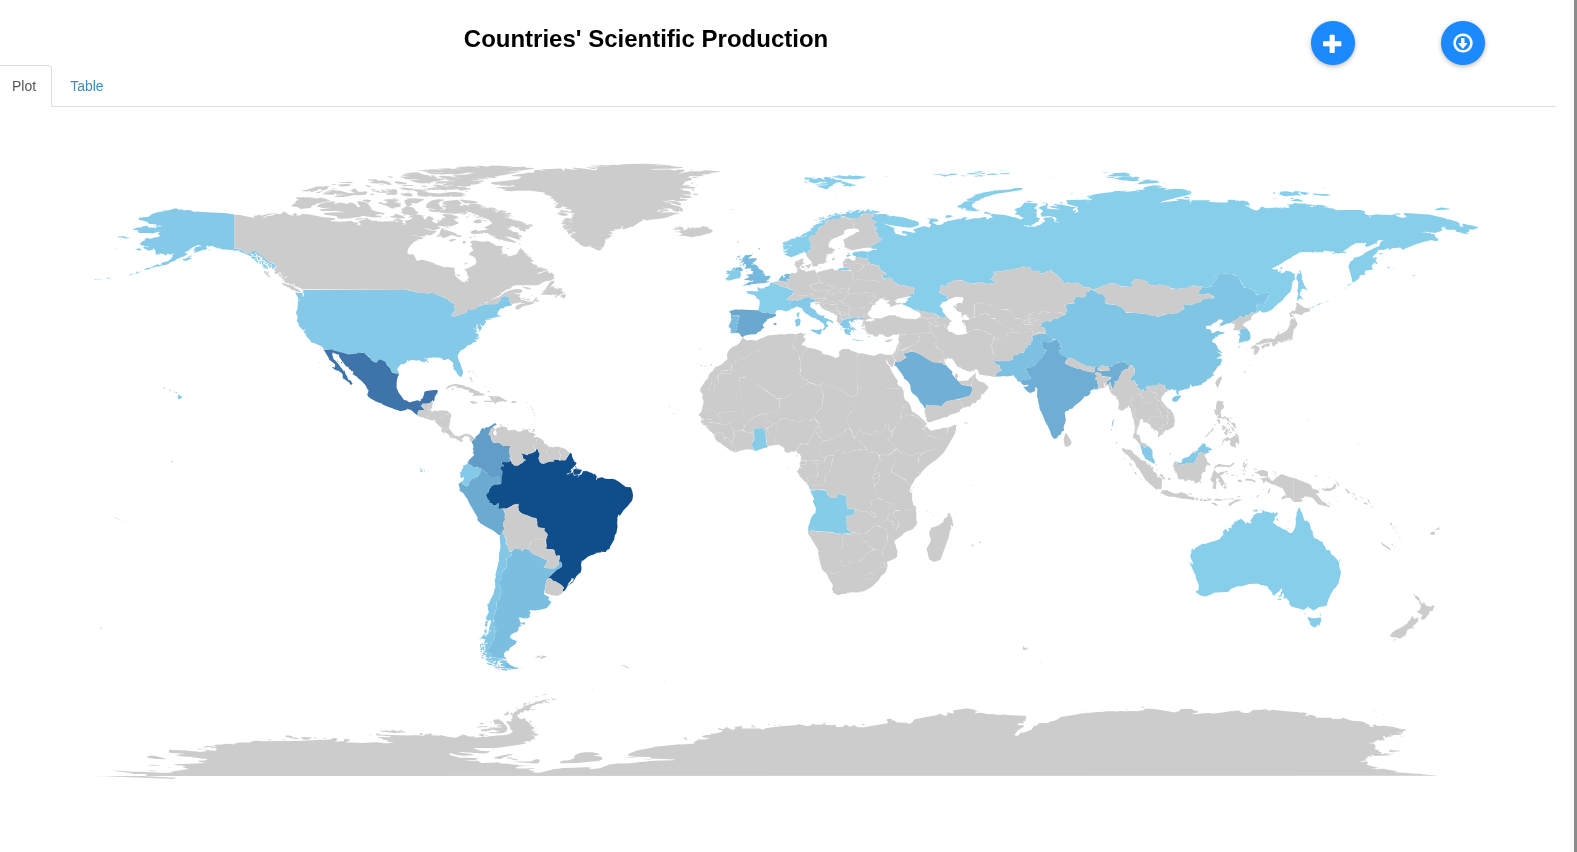
\includegraphics[width=0.8\textwidth]{Images/MapaBibliometrix.png}
\end{adjustbox}

\paragraph{Gráfico de Líneas:}
El gráfico de líneas detalla la tendencia de la producción científica a lo largo del tiempo para varios países seleccionados. Se puede observar un crecimiento generalizado en el número de artículos publicados, lo que refleja una expansión del campo de estudio. Países como Brasil y México muestran un incremento sustancial en la producción en los últimos años, lo que podría indicar un aumento en la inversión en investigación o un mayor enfoque en el tema. Por otro lado, países como Peru exhiben un crecimiento más moderado. 

Es crucial analizar estos datos en el contexto de factores como políticas de investigación nacionales, financiamiento disponible y colaboración internacional para comprender las dinámicas detrás de estas tendencias. 

\begin{adjustbox}{
    center,
    caption=[{Grafico de Lineas tomado de Bibliometrix}]{\centering Grafico de Lineas tomado de Bibliometrix},
    label={Grafico de Lineas tomado de Bibliometrix},
    nofloat=figure, vspace={7px}}
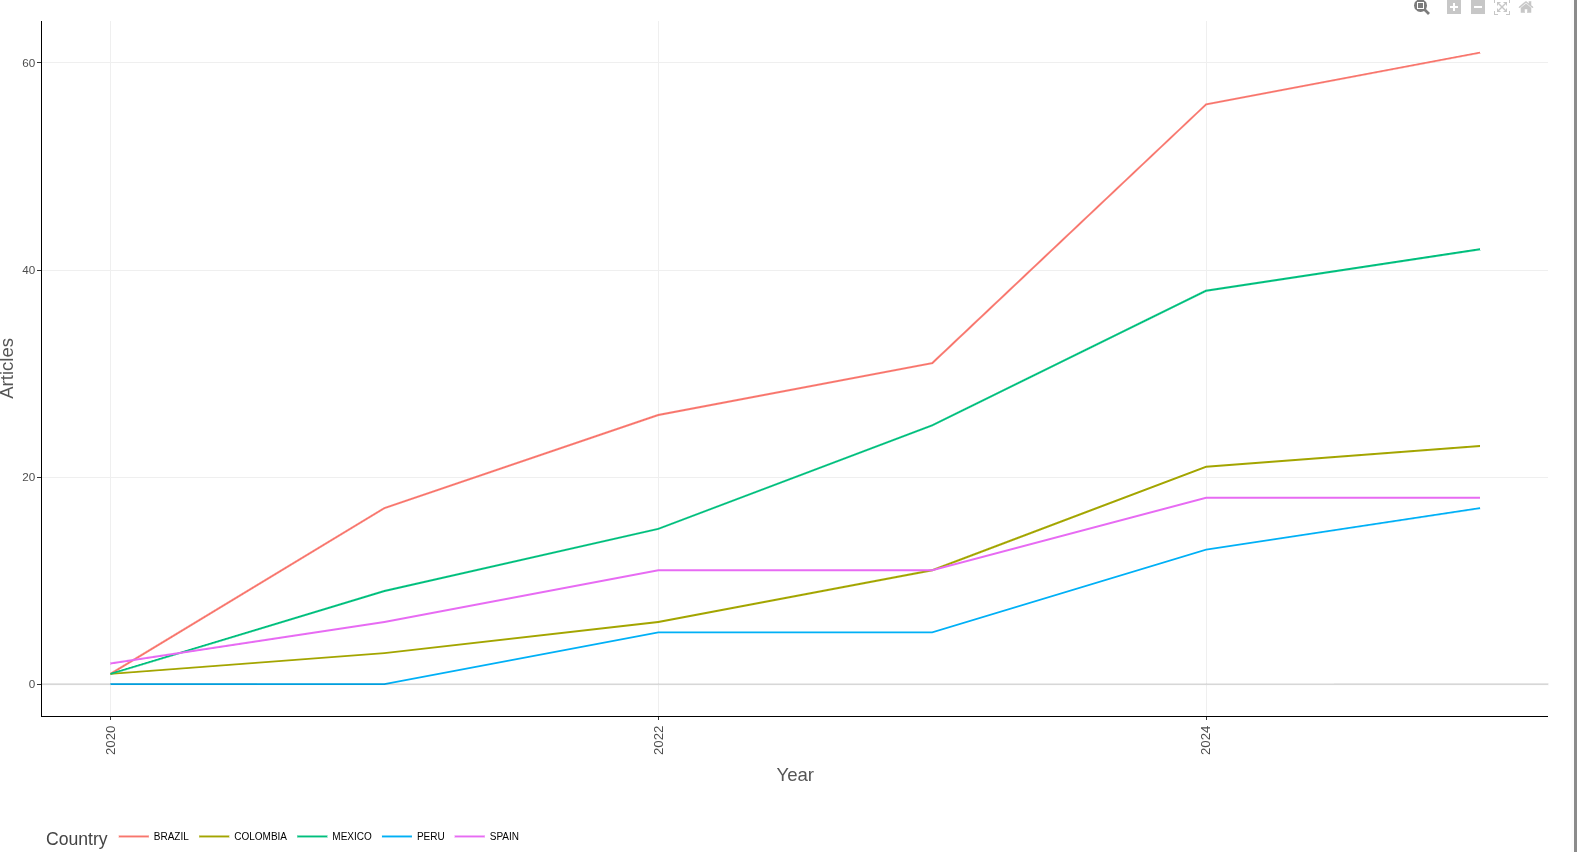
\includegraphics[width=0.8\textwidth]{Images/GraficoLineas.png}
\end{adjustbox}

\paragraph{Nube de Palabras (Word Cloud)}
\textbf{Descripción General:} Una nube de palabras representa visualmente la frecuencia con la que aparecen ciertas palabras en un texto o conjunto de textos. Las palabras más grandes indican una mayor frecuencia o importancia. 

\paragraph{Análisis Detallado y Texto Explicativo: }
La nube de palabras ofrece una visión rápida de los términos más relevantes en el conjunto de datos analizado. Las palabras de mayor tamaño, como 'blockchain', 'technology', 'system', 'management', 'network', 'design', 'framework', 'electronic medical-records', 'traceability', 'secure', 'privacy', 'distributed', 'information-management', 'challenges', 'optimization', 'internet', 'things' y 'encryption', señalan los temas centrales y las áreas de enfoque predominantes en la literatura. Esto sugiere un fuerte énfasis en los aspectos técnicos de blockchain, así como en sus aplicaciones en áreas como la gestión de información, la seguridad, la privacidad y los registros médicos electrónicos. 

La presencia de términos como 'challenges' y 'optimization' indica que la investigación también aborda los problemas y las mejoras potenciales de las tecnologías blockchain. La coexistencia de 'internet' y 'things' sugiere una conexión con el Internet de las Cosas (IoT) y su integración con blockchain. 

\begin{adjustbox}{
    center,
    caption=[{Nube de Palabras tomado de Bibliometrix}]{\centering Nube de Palabras tomado de Bibliometrix},
    label={Nube de Palabras tomado de Bibliometrix},
    nofloat=figure, vspace={7px}}
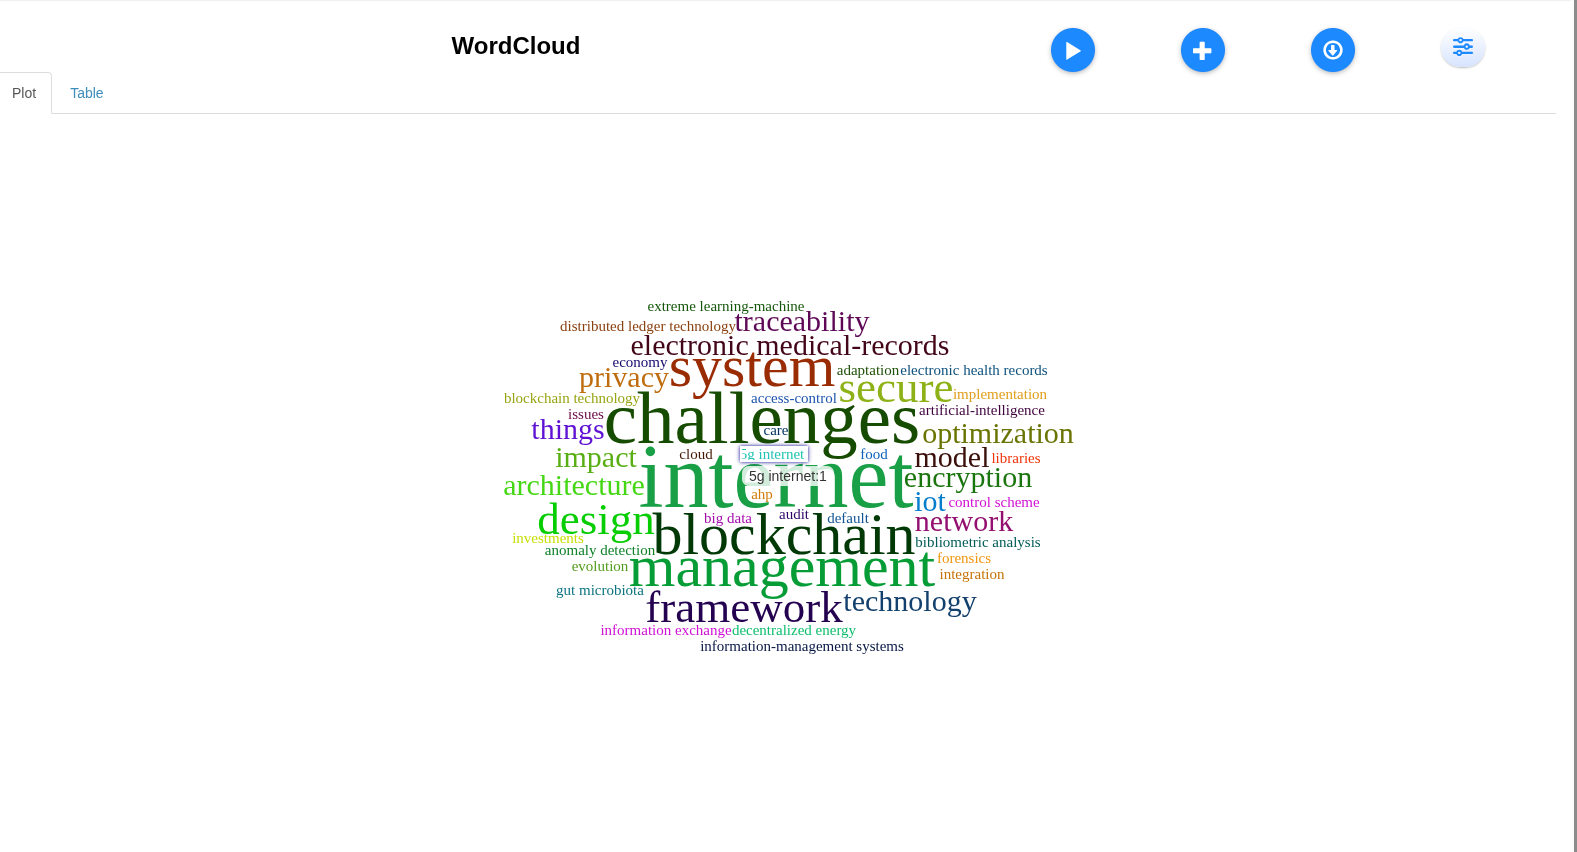
\includegraphics[width=0.8\textwidth]{Images/NubePalabras.png}
\end{adjustbox}

\paragraph{Mapa Temático (Thematic Map) }
\textbf{Descripción General:} Un mapa temático es una representación visual de los temas clave en un conjunto de documentos, organizado según su centralidad (relevancia) y densidad (desarrollo).  Los temas se representan como círculos, y su posición en el mapa indica su importancia y grado de desarrollo. 

\paragraph{Análisis Detallado y Texto Explicativo: }
El mapa temático clasifica los temas de investigación según su centralidad y densidad. Los temas ubicados en el cuadrante superior derecho, como 'Challenges framework electronic medical-records', son temas motores: están bien desarrollados y son importantes para el campo. Esto sugiere un enfoque significativo en los desafíos y marcos de trabajo relacionados con la aplicación de blockchain en los registros médicos electrónicos. 

Los temas en el cuadrante superior izquierdo, como 'system encryption', son temas muy desarrollados, pero menos centrales. Esto podría indicar áreas de investigación maduras que proporcionan la base teórica o metodológica para otros temas. Los temas en el cuadrante inferior derecho, como 'management secure network', son temas emergentes y centrales, lo que señala áreas de creciente interés e importancia para futuras investigaciones. El tema 'blockchain', ubicado en el cuadrante inferior izquierdo, es un tema básico, fundamental pero menos desarrollado en comparación con otros, lo que sugiere que es una tecnología fundacional que sustenta diversas áreas de investigación. 

El tema 'design impact traceability' se encuentra en el centro, lo que podría indicar que actúa como un tema puente que conecta diferentes áreas de investigación. 

\begin{adjustbox}{
    center,
    caption=[{Mapa Temático tomado de Bibliometrix}]{\centering Mapa Temático tomado de Bibliometrix},
    label={Mapa Temático tomado de Bibliometrix},
    nofloat=figure, vspace={7px}}
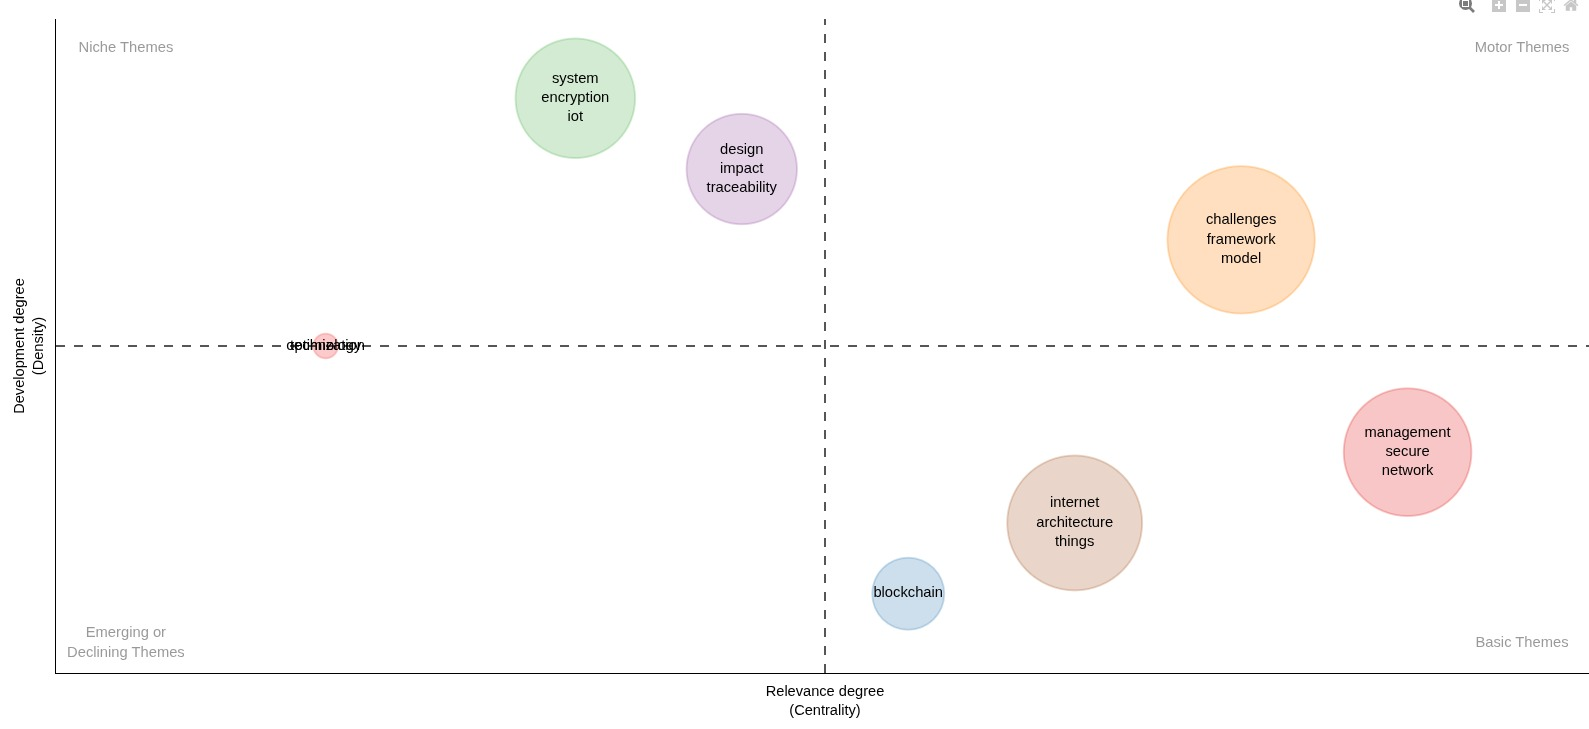
\includegraphics[width=0.8\textwidth]{Images/MapaTematico.jpeg}
\end{adjustbox}


 \section{Alcance}
 El ámbito de aplicación de este estudio y desarrollo de prototipo se delimita estrictamente al entorno operativo y regulatorio de la Secretaría Distrital de Movilidad de Bogotá. Esta focalización geográfica y contextual se justifica por la heterogeneidad de los sistemas de gestión de infracciones a nivel regional en Colombia, permitiendo así un análisis pertinente y detallado. Consecuentemente, el diseño y la evaluación del prototipo adoptarán la perspectiva de la entidad administradora, con énfasis en asegurar la integridad registral, la cadena de custodia de la evidencia y la auditabilidad del sistema. La arquitectura tecnológica propuesta se basa en la utilización de Hyperledger Fabric para el registro distribuido y el sistema IPFS para el almacenamiento de evidencia, cuya funcionalidad y características de rendimiento básicas serán objeto de validación mediante pruebas en un ambiente controlado, verificando la operatividad del flujo propuesto y la inmutabilidad de la información registrada. 

  \section{Metodología }
  La metodología de este proyecto se divide en dos componentes principales: la metodología de investigación y la metodología de desarrollo de software.  

    \subsection{Metodología de investigación }
 La metodología de investigación se clasifica de la siguiente manera: a) Por la forma en que la investigación es usada: El siguiente proyecto desea dar solución a los problemas que presenta la falta de seguridad en la gestión de 25 infracciones de tránsito en la Municipalidad Provincial del Cusco. Por lo tanto, es considerado como una investigación APLICADA. Siendo la definición: "La investigación Aplicada o Técnica tiende a la resolución de problemas o al desarrollo de ideas, dirigidas a conseguir innovaciones, mejoras de procesos o productos, etc." (Sanchez, 2011). b) Por el propósito del estudio: El presente proyecto realizará la identificación de las características más sobresalientes de la implementación de un Servicio Web con Blockchain, destacando los aspectos más sobresalientes para la mejora en la seguridad de gestión de infracciones de tránsito en la Municipalidad Provincial del Cusco. Por lo tanto, es considerada como DESCRIPTIVA. Siendo la definición: "Los estudios descriptivos buscan especificar las propiedades, las características y los aspectos importantes del fenómeno que se somete a análisis" (Gomez, 2006) 

   \subsection{Metodología de desarrollo de software: Enfoque por Prototipos }
Para el desarrollo de este proyecto, se adoptará la Metodología de Desarrollo por Prototipos. Esta elección se fundamenta en la naturaleza innovadora del proyecto, que combina tecnologías emergentes como Blockchain e IPFS en un dominio específico (gestión de fotocomparendos), donde los requisitos exactos y los desafíos técnicos pueden no ser completamente evidentes desde el inicio. La metodología por prototipos es inherentemente iterativa y se centra en la construcción rápida de versiones funcionales (prototipos) del sistema, permitiendo la validación temprana de conceptos, la recopilación de retroalimentación continua y la adaptación flexible a los descubrimientos realizados durante el desarrollo. 

\section{Diseño del Prototipo }
    \subsection{Definición de Requisitos:  }
    
\begin{enumerate}
    \item \textbf{Datos sobre infracciones de tráfico:} La captura de datos detallados sobre infracciones de tráfico, como la hora de la infracción, las coordenadas GPS, el tipo de infracción, los datos de identificación del vehículo e imágenes o vídeos, garantiza que cada incidente se documenta exhaustivamente. Este registro exhaustivo proporciona transparencia y responsabilidad, ya que los datos son inmutables y a prueba de manipulaciones una vez almacenados en la cadena de bloques. La inclusión de pruebas mediáticas refuerza aún más la credibilidad y verificabilidad de cada infracción, haciendo que los registros sean sólidos a efectos legales y administrativos. 
    \item \textbf{Información sobre el conductor:} Asociar las infracciones de tráfico a conductores concretos utilizando su dirección Ethereum (clave pública), los datos KYC si es necesario, y los números de identificación del conductor permite un seguimiento y una rendición de cuentas precisos. Esta vinculación de permite al sistema personalizar el seguimiento y la verificación de las sanciones, garantizando que las sanciones se atribuyan correctamente a las personas adecuadas. El uso de datos KYC garantiza que las identidades de los conductores puedan verificarse de forma fiable en, lo que resulta esencial para mantener la integridad y fiabilidad del sistema.
    \item \textbf{Datos de la sanción: }  Registrando los datos de la sanción, incluyendo el tipo de sanción, el importe de la sanción y el estado del pago de la sanción facilita la ejecución automatizada de las sanciones a través de contratos inteligentes. Esta automatización reduce la carga administrativa de y garantiza que las sanciones se apliquen de forma coherente y transparente. El registro inmutable de las sanciones y su estado de pago en la blockchain garantiza que el proceso sea justo y responsable, proporcionando una pista de auditoría clara para todas las transacciones financieras relacionadas con las infracciones de tráfico.
        \item \textbf{Eventos de contratos inteligentes:} El registro de eventos de contratos inteligentes, como el registro de nuevas infracciones de tráfico o la ejecución de sanciones, con datos relevantes y marcas de tiempo, garantiza que todas las acciones significativas se documenten de forma transparente. Este registro de eventos mejora la trazabilidad y la rendición de cuentas, proporcionando un registro cronológico de las actividades importantes del sistema. Esta transparencia es crucial para las auditorías y revisiones, ya que ayuda a a generar confianza en las operaciones del sistema. 
        \item \textbf{Datos de las transacciones de la cadena de bloques: } El seguimiento de los datos de las transacciones de la cadena de bloques, incluido el hash de la transacción, las direcciones del remitente/receptor y las tarifas del gas, proporciona un registro detallado de todas las interacciones dentro del sistema. Estos datos permiten supervisar y auditar las transacciones, garantizando la transparencia y la trazabilidad. Además, hacer un seguimiento de las tarifas de gas ayuda a gestionar y optimizar los costes asociados a la ejecución de transacciones en la blockchain, que es importante para mantener la rentabilidad del sistema. 
        \item \textbf{Dispositivos de datos IoT:} La integración de datos de dispositivos IoT, como sensores o cámaras, junto con marcas de tiempo e identificación del dispositivo, puede mejorar las pruebas recopiladas para infracciones de tráfico. Estos datos en tiempo real proporcionan a contexto adicional y pruebas corroborativas, haciendo que los registros de infracciones sean más sólidos y fiables. El uso de dispositivos IoT también puede automatizar la detección y el registro de infracciones, aumentando la eficiencia y la precisión del sistema.
            \item \textbf{Opiniones de los usuarios: } La recopilación de opiniones de los usuarios, incluidos el tipo de opinión, los comentarios y las valoraciones de los usuarios, ayuda a los administradores del sistema a comprender las experiencias y percepciones de los usuarios. Esta información es valiosa para identificar áreas de mejora en y mejorar la usabilidad y funcionalidad del sistema. Involucrar a los usuarios de esta manera puede conducir a un diseño del sistema más centrado en el usuario, mejorando la satisfacción y la eficacia general. 
                \item \textbf{Datos de cumplimiento: } El registro de los datos de cumplimiento, incluido el estado de cumplimiento y los detalles normativos, garantiza que el sistema se adhiere a las leyes y normativas de tráfico locales. Este seguimiento es vital para demostrar el cumplimiento de la normativa y evitar problemas legales. El mantenimiento de registros de cumplimiento detallados también facilita las auditorías reglamentarias en, proporcionando pruebas transparentes de que el sistema funciona dentro de las normas legales, lo que es esencial para generar confianza y credibilidad entre las partes interesadas.
\end{enumerate}

\subsection{Diagrama de casos de uso del sistema de gestión de infracciones de transito }
% img
\begin{adjustbox}{
    center,
    caption=[{Casos de Uso.}]{\centering Casos de Uso},
    label={Casos de Uso},
    nofloat=figure, vspace={7px}}

    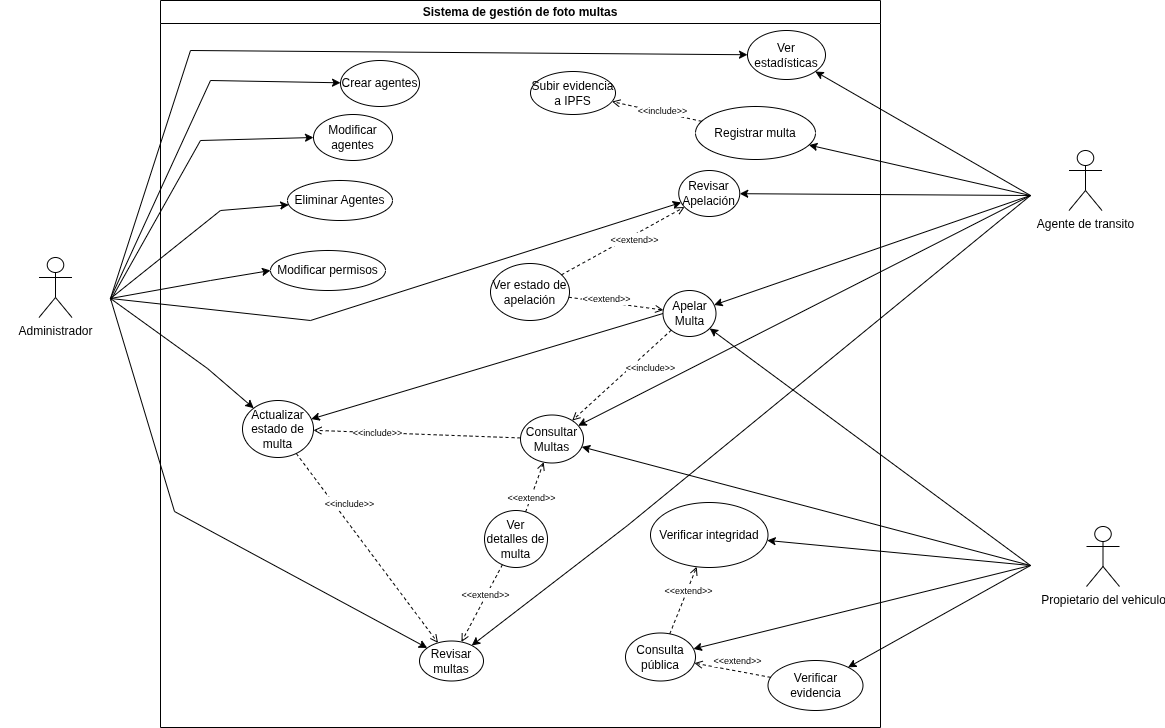
\includegraphics[width=0.8\textwidth]{Images/CasosUso.png}
\end{adjustbox}

 \subsection{ Diagrama de Despliegue }
\begin{adjustbox}{
    center,
    caption=[{Arquitectura}]{\centering Diagrama de Despliegue},
    label={DiagramaDespliegue},
    nofloat=figure, vspace={7px}}

    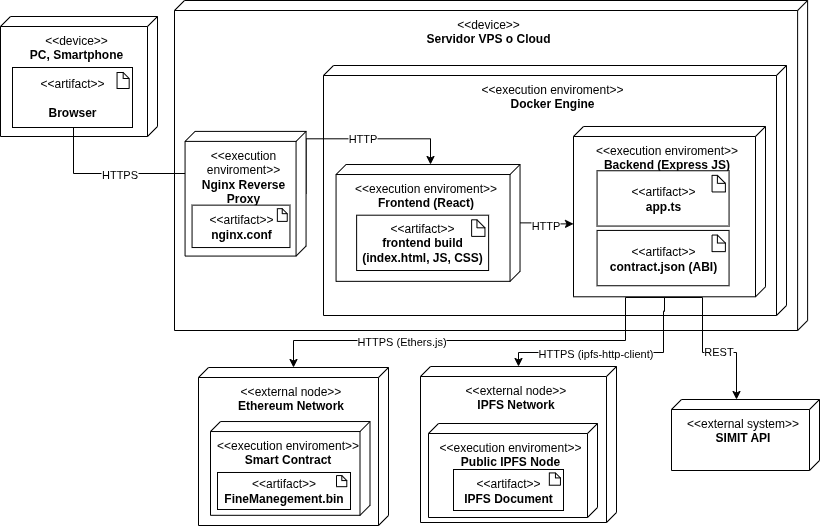
\includegraphics[width=0.8\textwidth]{Images/Despliegue.png}
\end{adjustbox}
En la Figura anterior se puede observar el diagrama de despliegue propuesto, donde cada nodo cuenta con la misma información, ya que esta se encontrará sincronizada. Así mismo, se encuentra conectada mediante Servicios Web a la base de datos de Apitude para como herramienta de terceros para acceder a la informacion existente en el Registro Único Nacional de Tránsito (RUNT) de donde se obtendrán los datos de conductores y vehículos y registro existente de infractores a nivel Bogotá y estado de las multas 

Hay que mencionar que existen dos soluciones para traer la información necesaria de estas entidades, la primera siendo un api llamado apitude de un tercero que trae la información del RUNT y del SIMIT, y segundo los datos que estas entidades públicas ya poseen en bases de datos tradicionales. 
 \subsection{ Diagrama de clases }
Hay que considerar que se manejaran dos capas de lógica la primera enfocada en registrar los cambios en los estados de las multas a raves de blockchain y la segunda capa de lógica que se encarga de la administración general de las multas (manipular los datos que no son visibles ante el público) 
 \begin{adjustbox}{
    center,
    caption=[{Diagrama de clases}]{\centering Diagrama de clases},
    label={Diagrama de clases},
    nofloat=figure, vspace={7px}}

    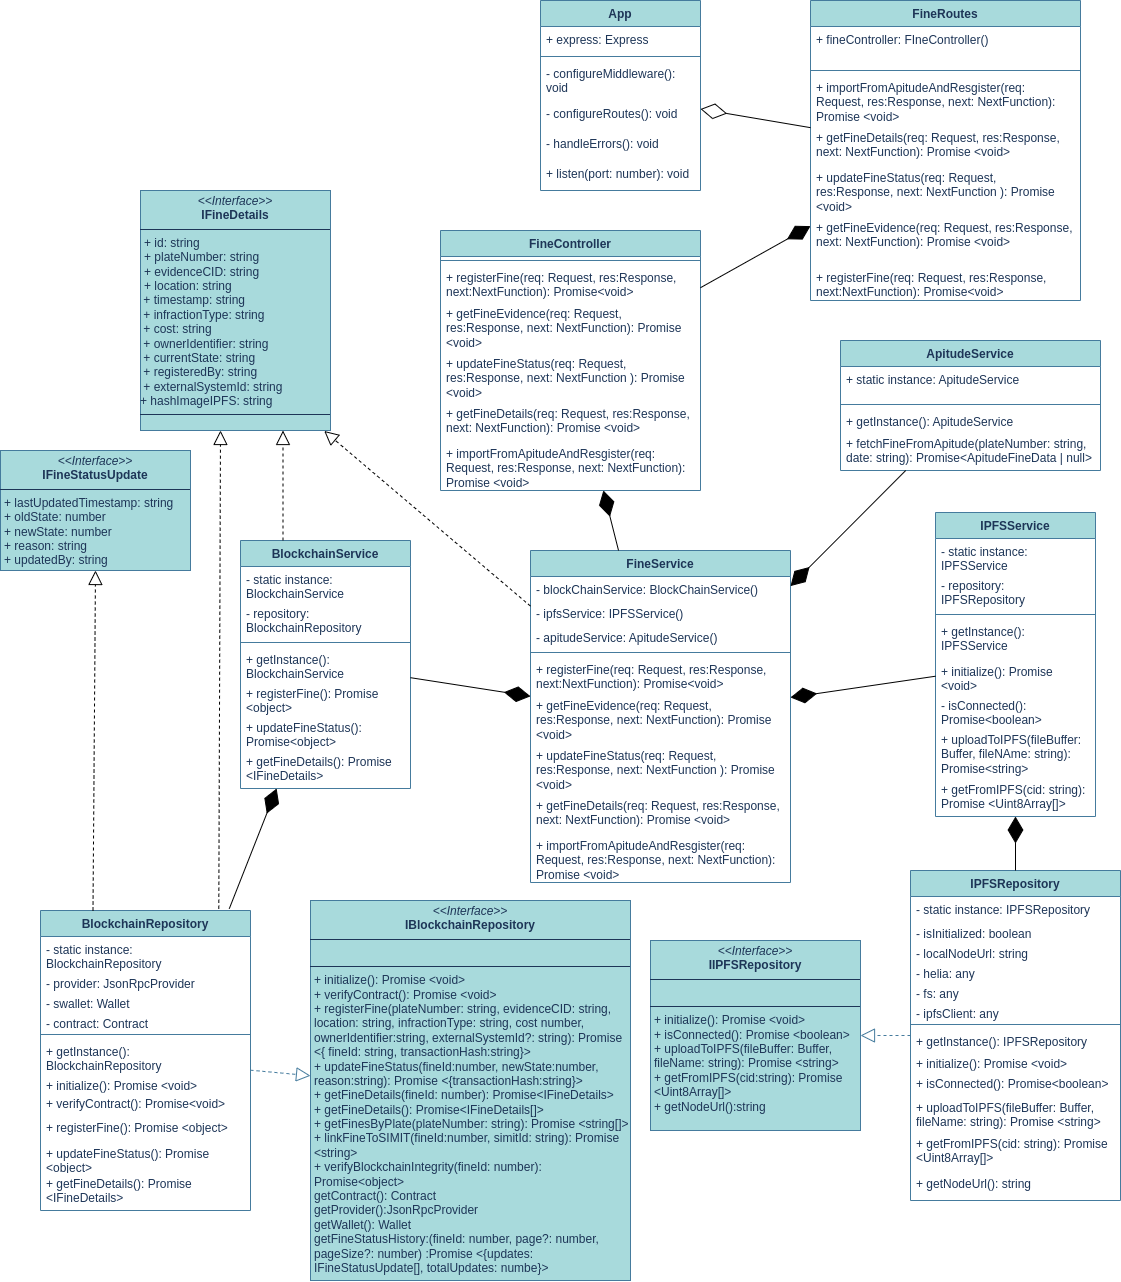
\includegraphics[width=0.8\textwidth]{Images/uml.png}
\end{adjustbox}
En la figura 3 se hace un esquema de la primera capa logica que se encarga de la administracion general de las multas y los datos que maneja
 \begin{adjustbox}{
    center,
    caption=[{Diagrama de clases part.2}]{\centering Diagrama de Apelacion de multa},
    label={DiagramaApelacionMulta2},
    nofloat=figure, vspace={7px}}
    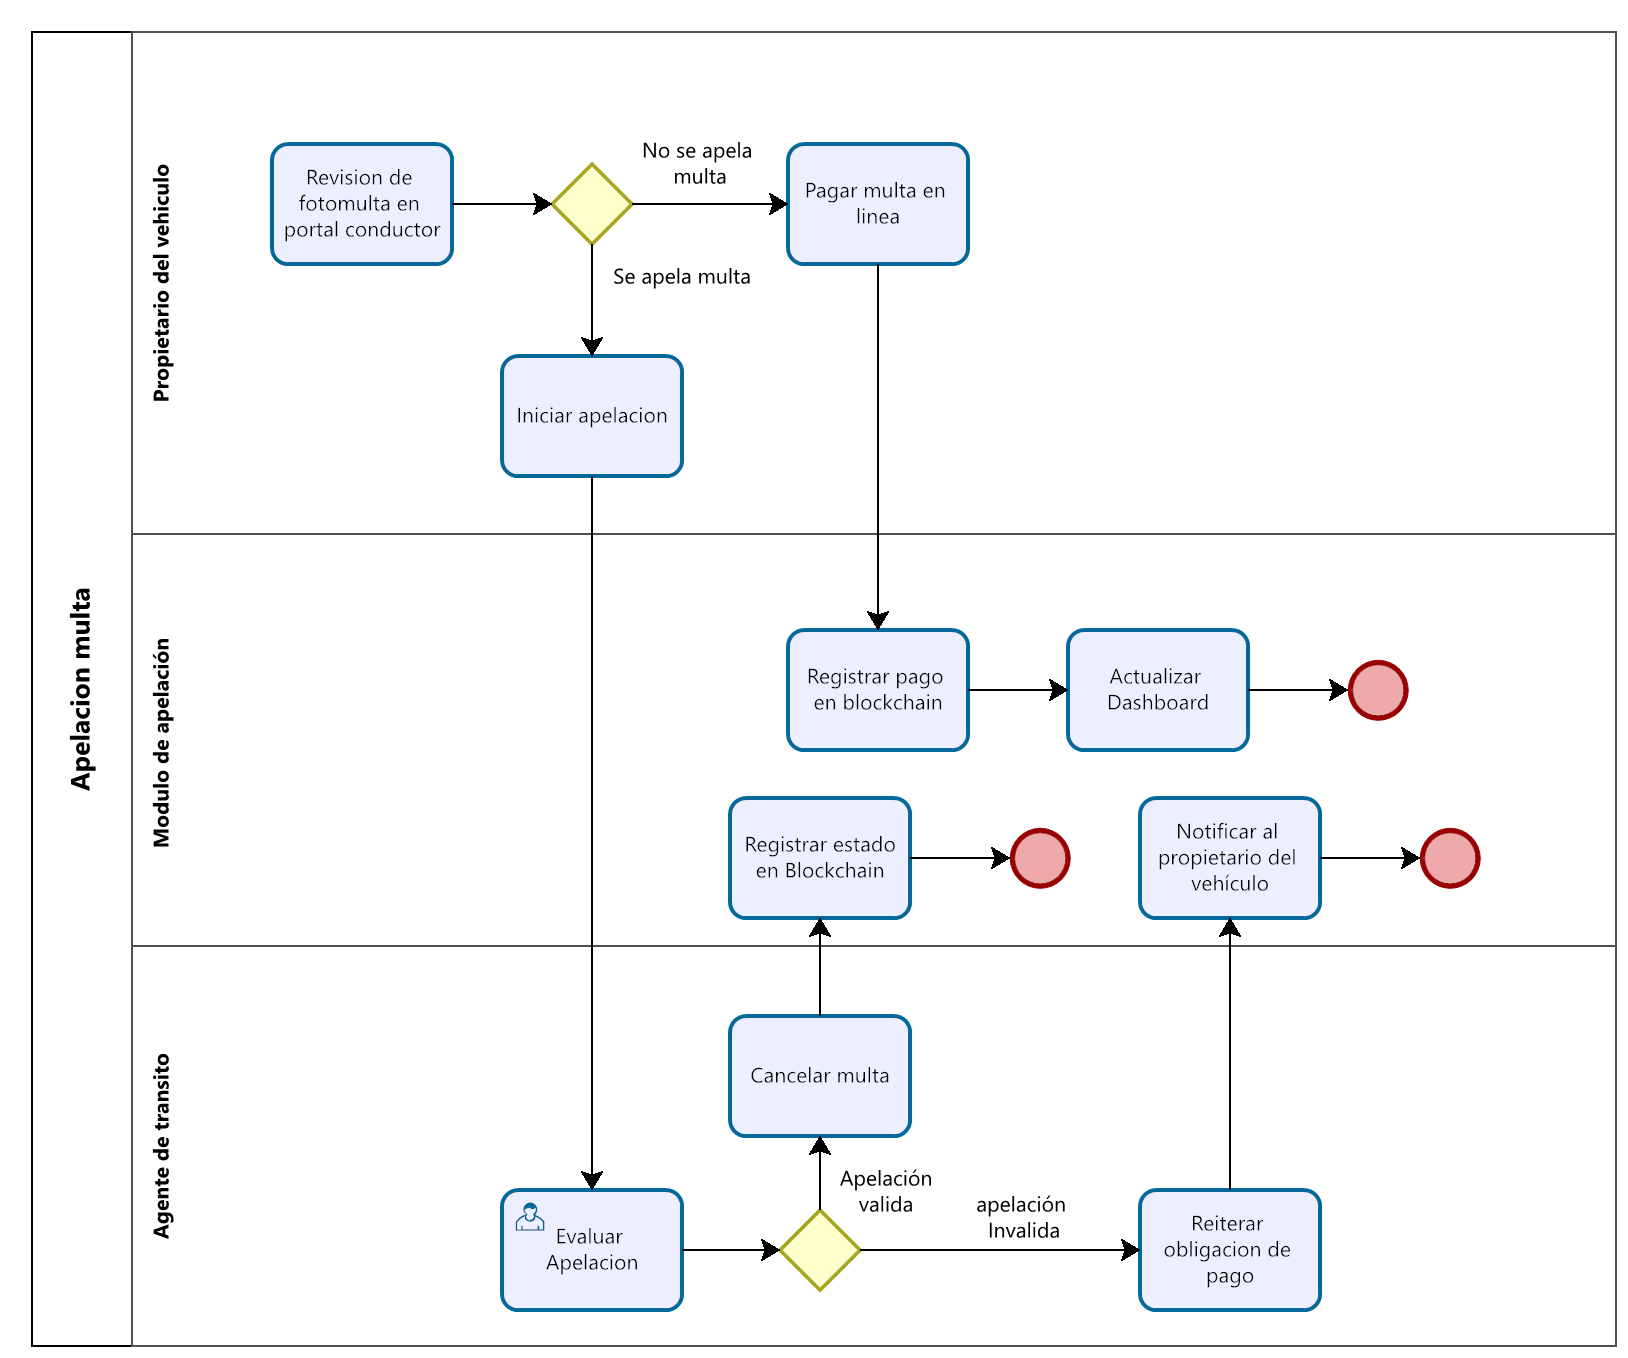
\includegraphics[width=0.8\textwidth]{Images/ActApelacion.png}
\end{adjustbox}
En la figura 4 se hace mención en la segunda capa lógica la cual son los cambios generados en el registro de multas que registramos en la blockchain, que se traducen en los contratos realizados en solidity.
\subsection{ Diagrama de actividades }
 \begin{adjustbox}{
    center,
    caption=[{Diagrama de clases part.2}]{\centering Diagrama de Creacion de multa},
    label={DiagramaCreacionMulta},
    nofloat=figure, vspace={7px}}
    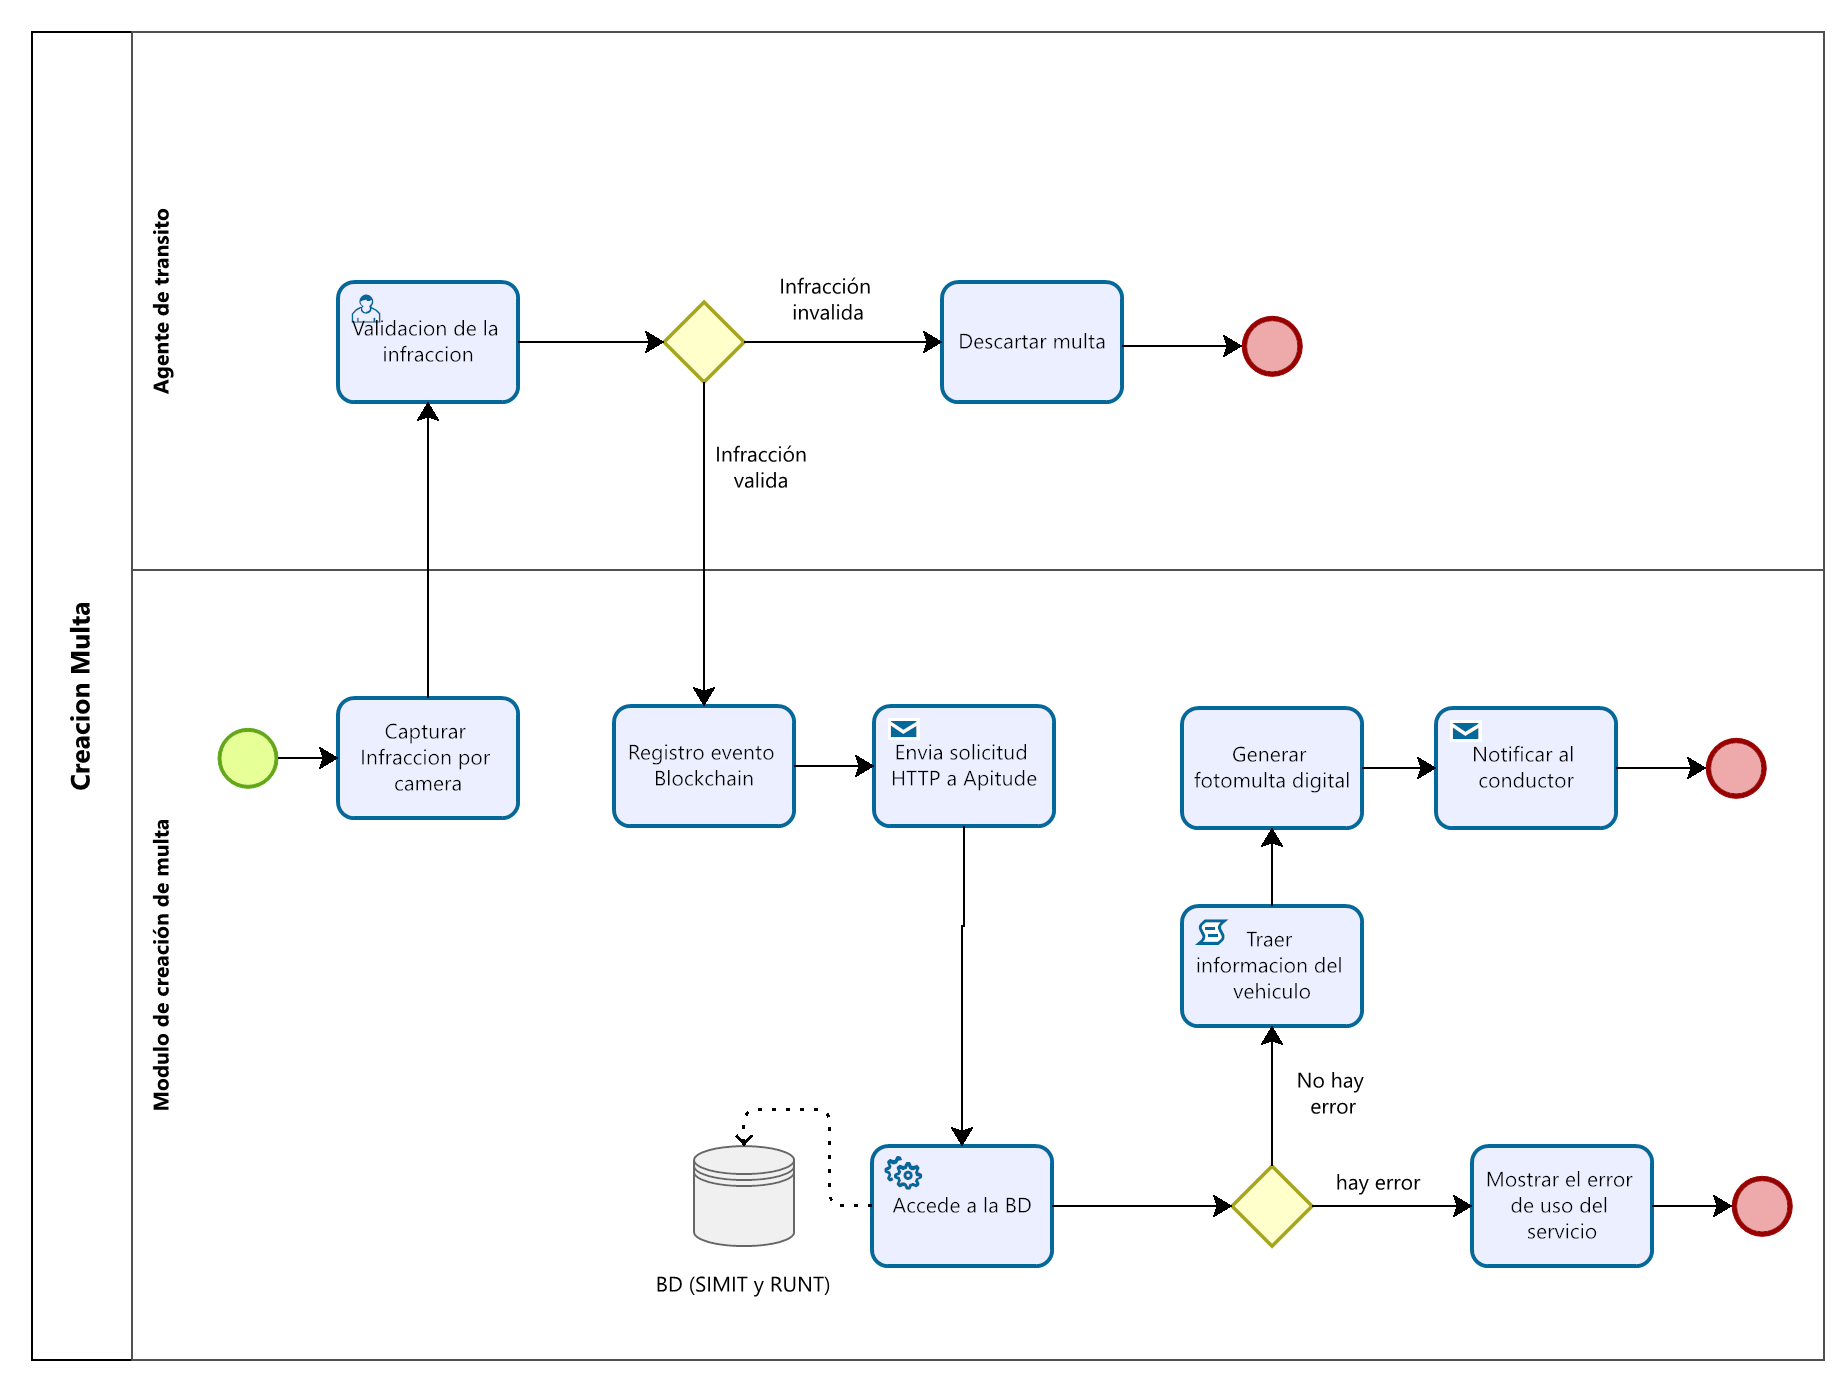
\includegraphics[width=0.8\textwidth]{Images/ActMulta.png}
\end{adjustbox}
 \begin{adjustbox}{
    center,
    caption=[{Diagrama de clases part.2}]{\centering Diagrama de Apelacion de multa},
    label={Diagrama de clases part.2},
    nofloat=figure, vspace={7px}}
    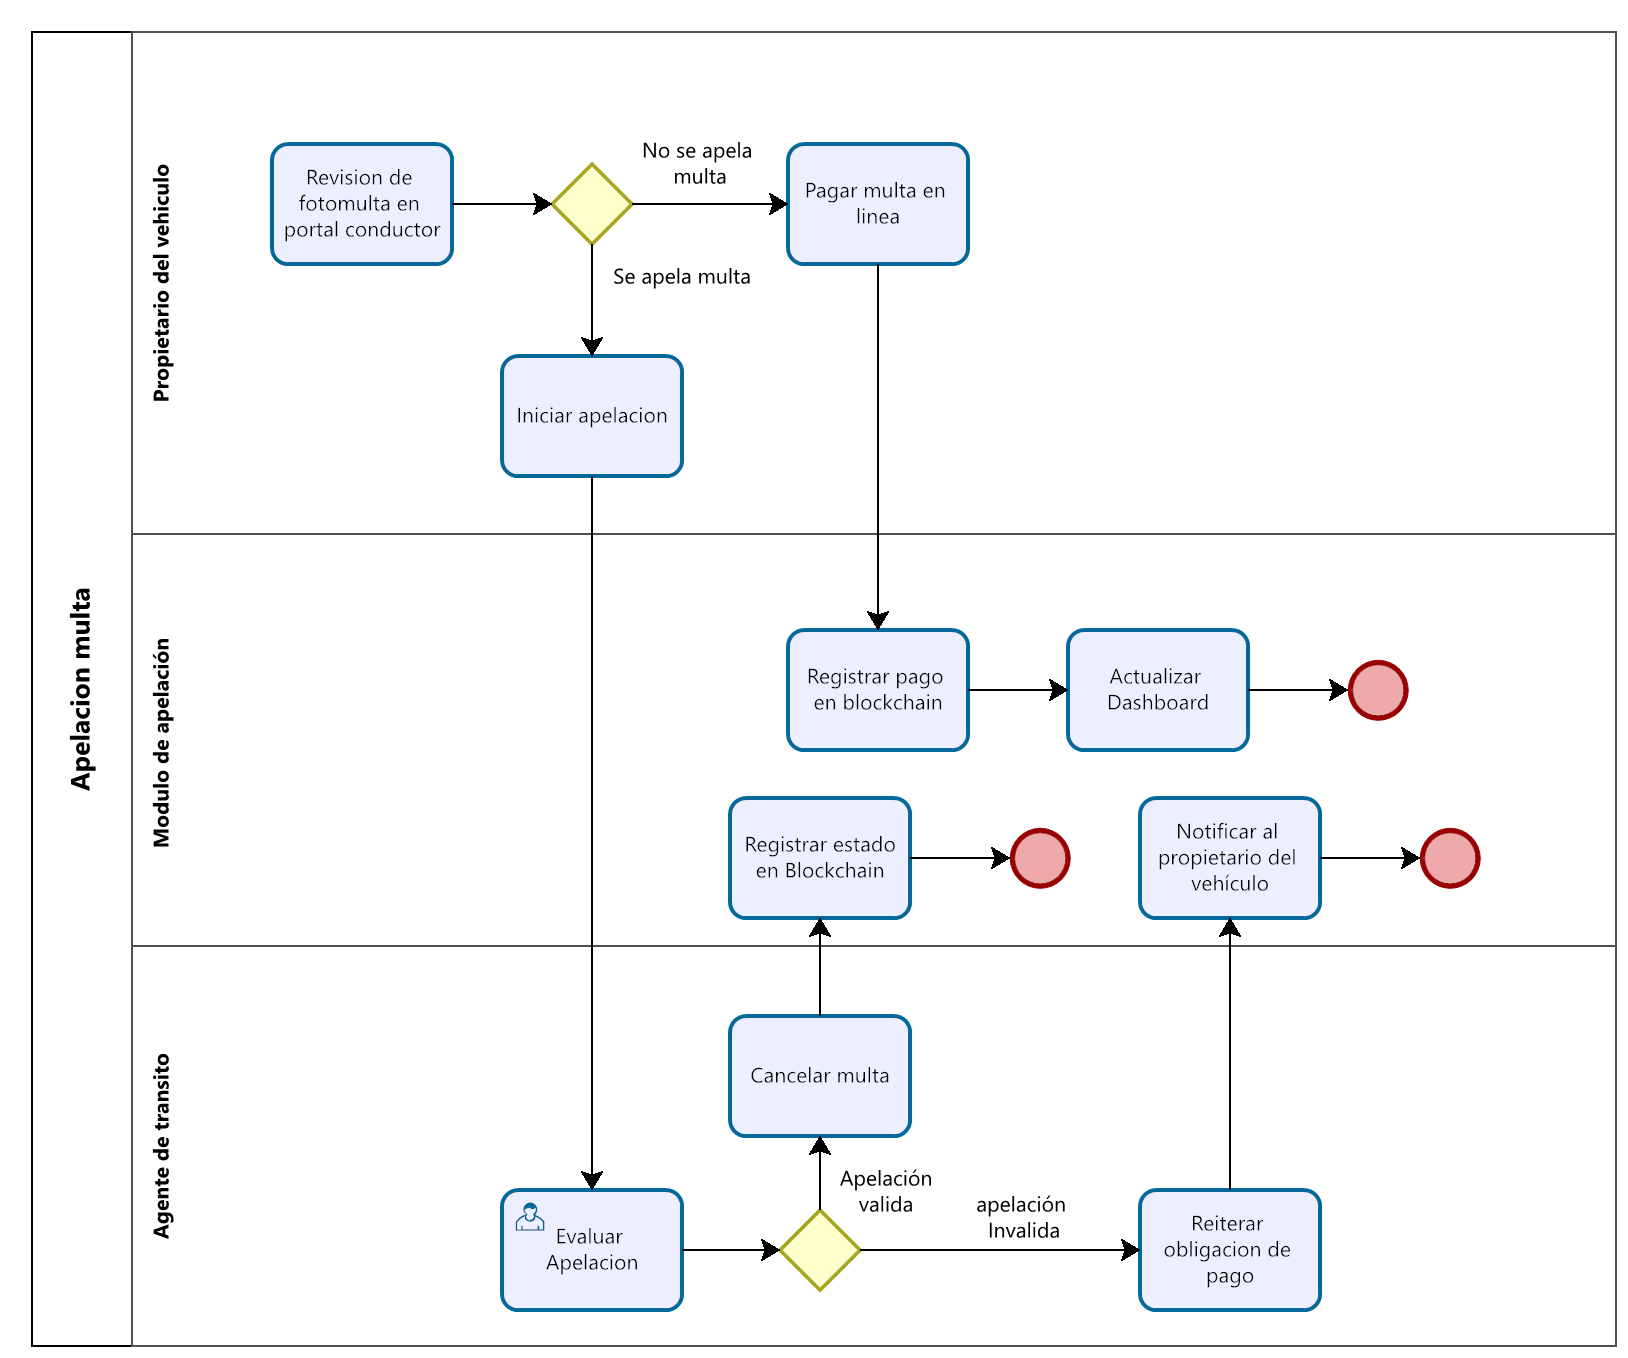
\includegraphics[width=0.8\textwidth]{Images/ActApelacion.png}
\end{adjustbox}

\subsection{Interfaz de Usuario}
\paragraph{Compartidas}
 \begin{adjustbox}{
    center,
    caption=[{Login}]{\centering Login},
    label={Login},
    nofloat=figure, vspace={7px}}
    
\includegraphics[width=0.8\textwidth]{Images/UI1.png}
\end{adjustbox}

 \begin{adjustbox}{
    center,
    caption=[{Recuperar Contraseña}]{\centering Recuperar Contraseña},
    label={Recuperar Contraseña},
    nofloat=figure, vspace={7px}}
    
\includegraphics[width=0.8\textwidth]{Images/UI2.png}
\end{adjustbox}
\paragraph{Vista Agente}
\begin{adjustbox}{
    center,
    caption=[{Dashboard Agente de transito }]{\centering Dashboard Agente de transito},
    label={Dashboard Agente de transito},
    nofloat=figure, vspace={7px}}
    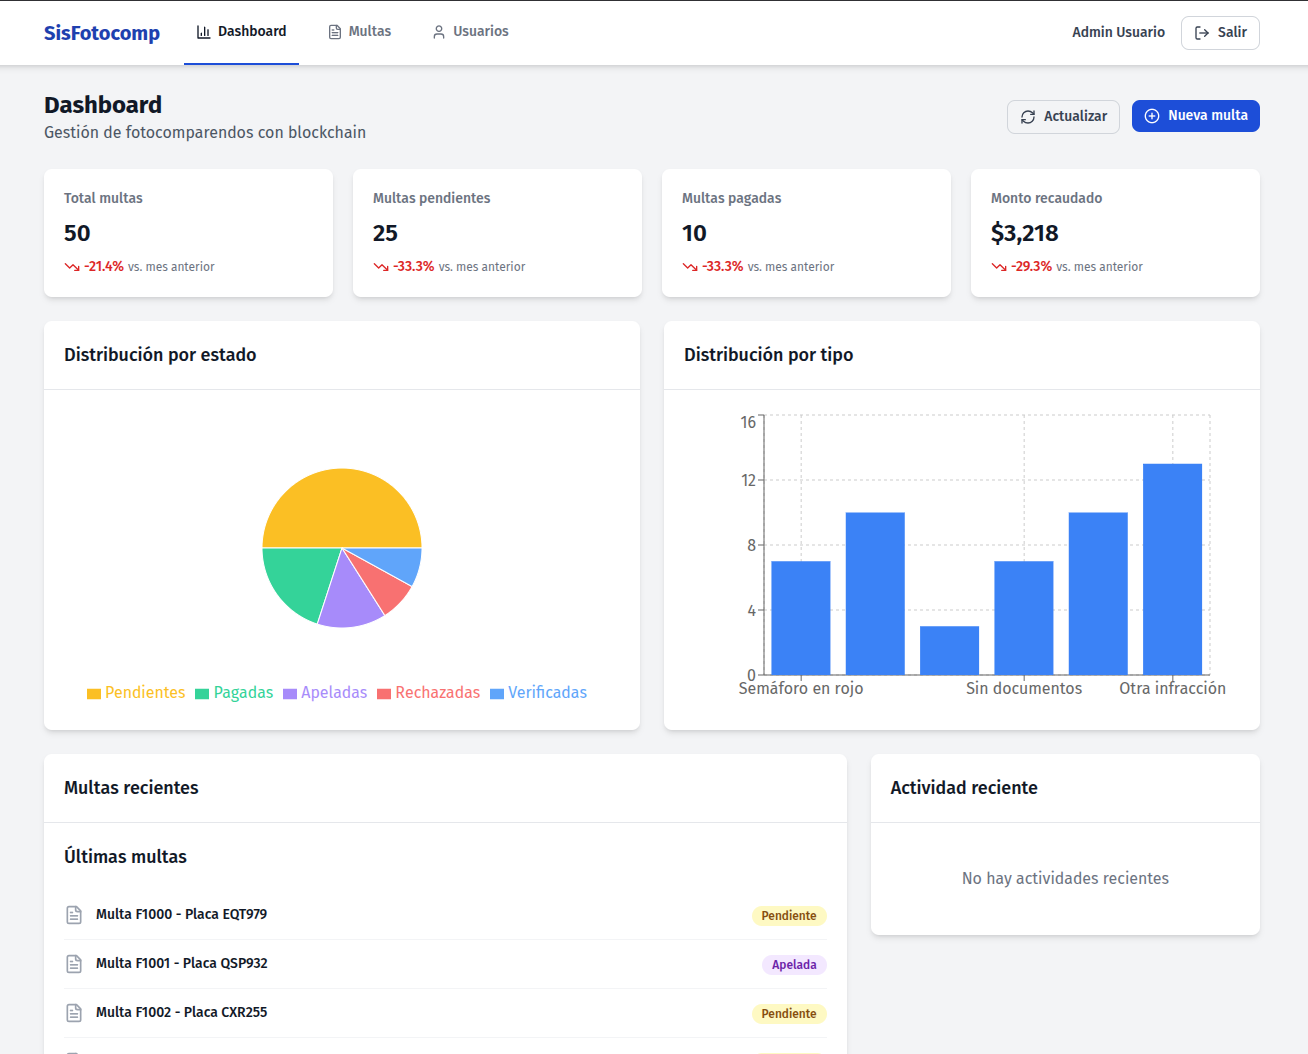
\includegraphics[width=0.8\textwidth]{Images/UI3.png}
\end{adjustbox}
\begin{adjustbox}{
    center,
    caption=[{Consulta Estado de multa}]{\centering Consulta Estado de multa},
    label={Consulta Estado de multa},
    nofloat=figure, vspace={7px}}
    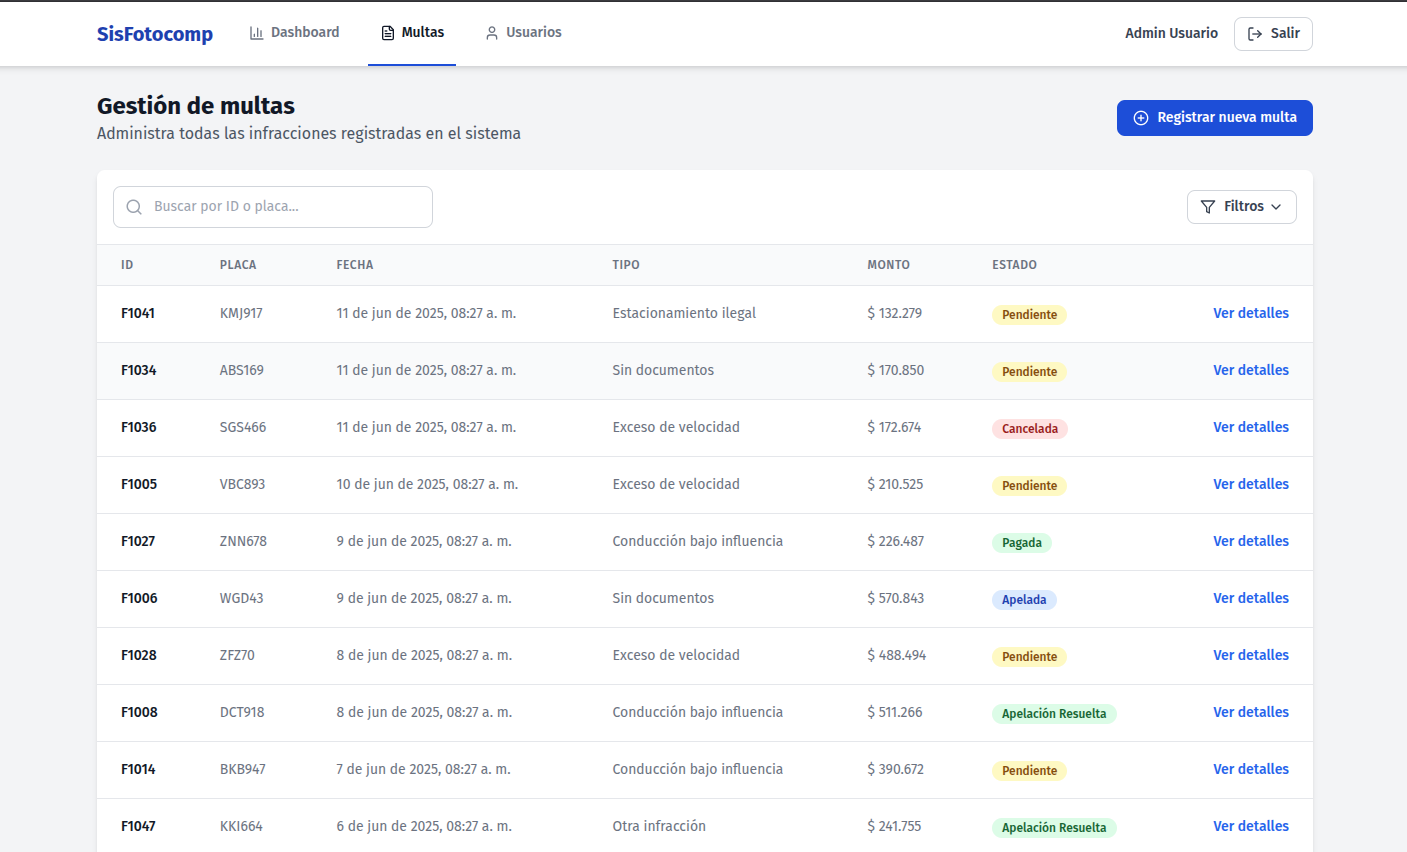
\includegraphics[width=0.8\textwidth]{Images/UI4.png}
\end{adjustbox}
\begin{adjustbox}{
    center,
    caption=[{Consulta Detalle de multa}]{\centering Consulta Detalle de multa},
    label={Consulta Detalle de multa},
    nofloat=figure, vspace={7px}}
    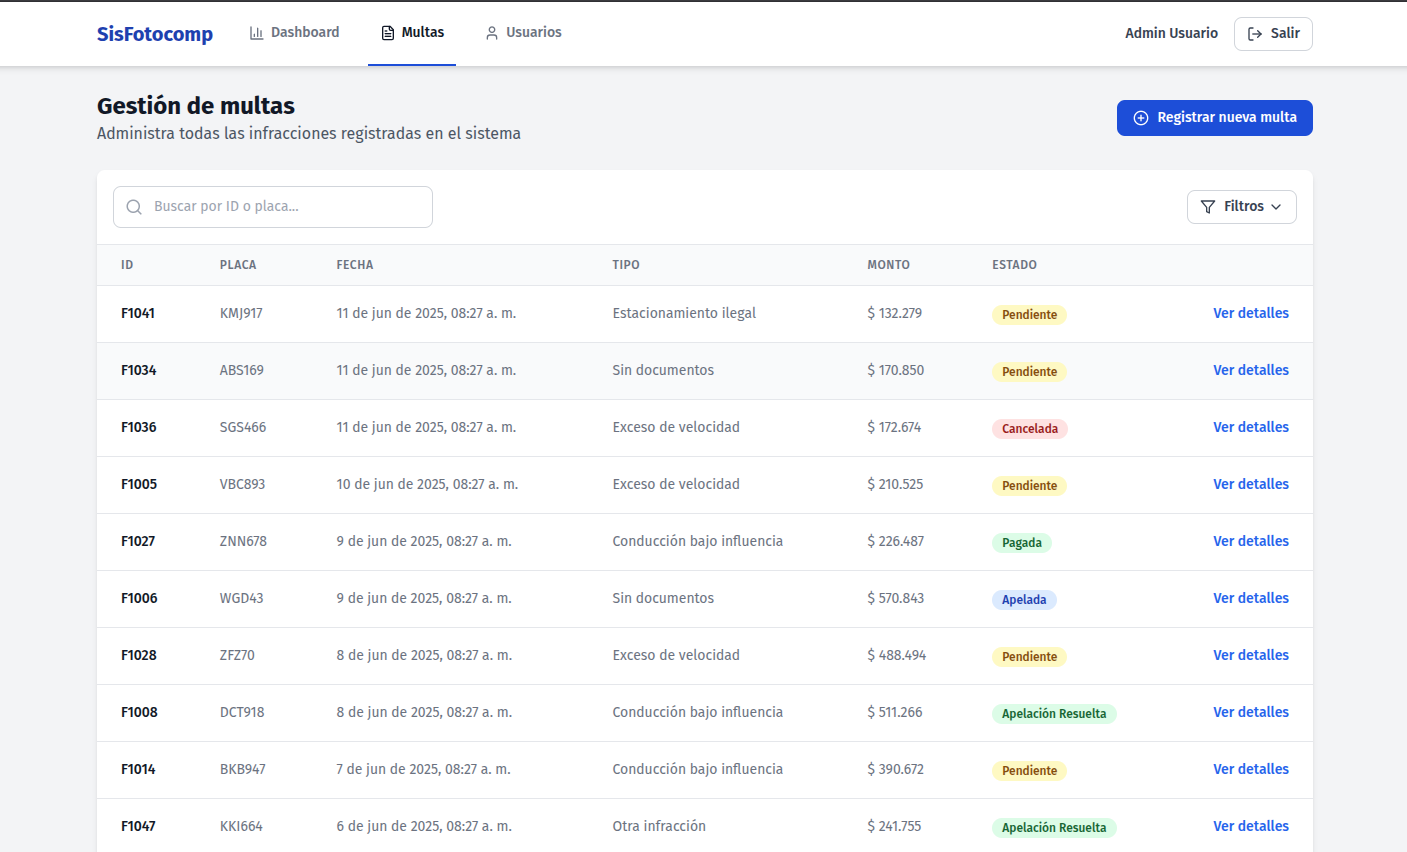
\includegraphics[width=0.8\textwidth]{Images/UI4.png}
\end{adjustbox}
\paragraph{Vista Propietario de Vehiculo}
\begin{adjustbox}{
    center,
    caption=[{Consulta multas}]{\centering Consulta multas},
    label={Consulta multas},
    nofloat=figure, vspace={7px}}
    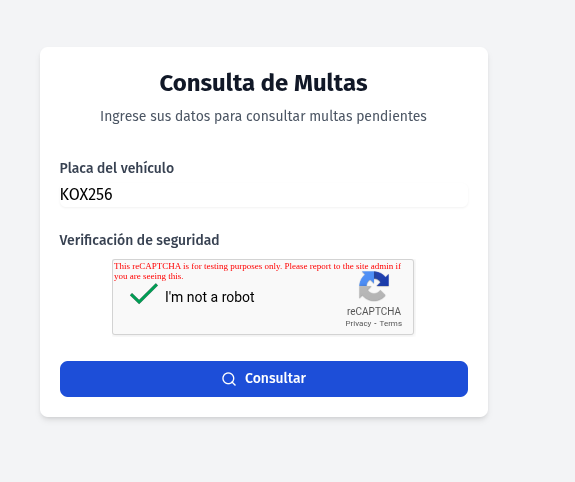
\includegraphics[width=0.8\textwidth]{Images/UI5.png}
\end{adjustbox}

\section{Costos del Proyecto}
\paragraph{Resumen de costos}

\begin{figure}[h!]
    \centering
    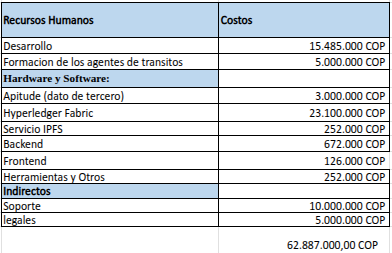
\includegraphics[width=\textwidth]{Images/costos1.png}
    \caption{Resumen de Costos del Proyecto.}
    \label{fig:costos1}
\end{figure}

Este proyecto involucra el desarrollo e implementación de un sistema de software complejo que utiliza tecnologías modernas como blockchain (Hyperledger Fabric) e IPFS, junto con componentes web tradicionales (React, Express.js). Los costos se han estimado cuidadosamente considerando el esfuerzo de desarrollo, la infraestructura necesaria, la capacitación y otros gastos indirectos. 

El costo total estimado del proyecto asciende a 62.887.000,00 COP. Este monto se desglosa en varias categorías principales que detallaremos a continuación, basándonos en una estimación ascendente del esfuerzo y una proyección de los costos de infraestructura y servicios. 

\paragraph{Costos de Software y Hardware}

\begin{figure}[h!]
    \centering
    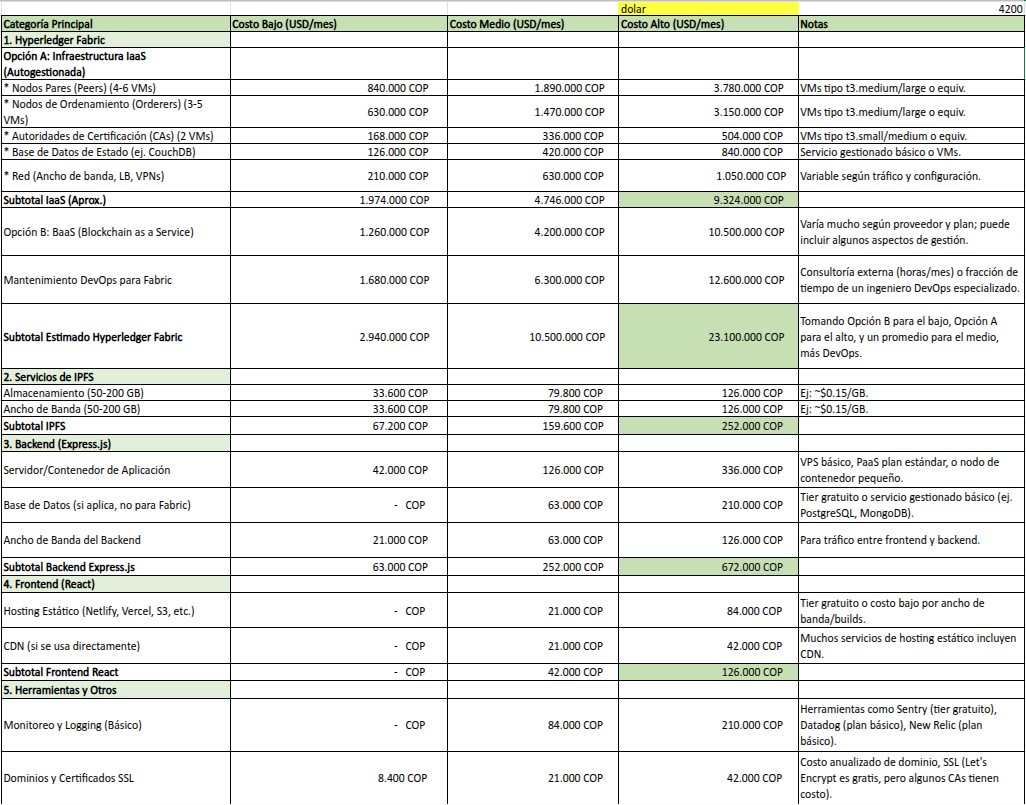
\includegraphics[width=\textwidth]{Images/costos2.png}
    \caption{Estimación de Costos Mensuales de Infraestructura.}
    \label{fig:costos2}
\end{figure}

Esta tabla proyecta los costos mensuales recurrentes asociados con la infraestructura necesaria para desplegar y operar la aplicación. Ofrece tres escenarios (Bajo, Medio, Alto) para cada componente, reflejando diferentes niveles de capacidad, rendimiento o robustez. Los valores en esta tabla están originalmente en dólares (USD) y se han convertido a pesos colombianos (COP) utilizando una tasa de cambio de 4.200 COP/USD (según la celda indicada). Se ha seleccionado el escenario "Costo Alto (USD/mes)" para alimentar la tabla de "Resumen de Costos". 

\paragraph{Categorías Principales y Subcomponentes (basado en el escenario "Alto" seleccionado): }

\begin{enumerate}
\item \textbf{Hyperledger Fabric:} Es el costo más significativo, reflejando la complejidad de desplegar y mantener una red blockchain permisionada. 

\begin{itemize}
\item \textbf{Infraestructura IaaS (Autogestionada) o BaaS:} Incluye servidores para nodos pares, nodos de ordenamiento, autoridades de certificación, bases de datos de estado y costos de red. El escenario alto seleccionado suma 9.324.000 COP. 

\item \textbf{Mantenimiento DevOps para Fabric:} Un costo crucial para la operación, monitoreo y actualización de la red Fabric, estimado en 12.600.000 COP. 

\item\textbf{Subtotal Estimado Hyperledger Fabric:} 23.100.000 COP (Nota: parece haber una pequeña diferencia entre la suma de los componentes IaaS y DevOps, y el subtotal. El subtotal de 23.100.000 COP es el que se traslada al resumen). 
\end{itemize}
\item \textbf{Servicios de IPFS:} Costos asociados al almacenamiento y ancho de banda para el 		sistema de archivos descentralizado, estimados en 252.000 COP. 

\item \textbf{Backend (Express.js):} Costos del servidor de aplicación, base de datos (si aplica fuera de Fabric) y ancho de banda para la API, sumando 672.000 COP. 

\item \textbf{Frontend (React):} Costos de hosting estático y CDN para la interfaz de usuario, estimados en 126.000 COP. 

\item \textbf{Herramientas y Otros:} Incluye monitoreo, logging, dominios y certificados SSL, con un costo de 252.000 COP. 
\end{enumerate}
 

\textbf{GRAN TOTAL ESTIMADO MENSUAL (Escenario Alto):} El costo mensual recurrente total para la infraestructura y servicios, en el escenario alto, es de 24.402.000 COP. Nota: Este es el costo mensual. En la tabla de resumen de costos, algunos de estos se presentan como si fueran un costo único o para un periodo específico, lo cual habría que aclarar (ej. si el costo de Hyperledger Fabric de 23.100.000 COP es para el primer mes, o para un periodo de setup y algunos meses de operación). Si es mensual, el total del proyecto se dispararía si es para muchos meses. 

\paragraph{Costo de Desarrollo }
\begin{figure}[h!]
    \centering
    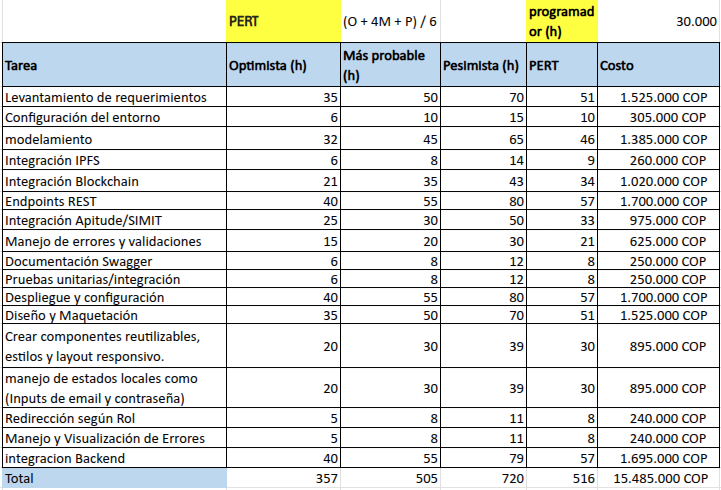
\includegraphics[width=\textwidth]{Images/costos3.png}
    \caption{Estimación de Costos de Desarrollo.}
    \label{fig:costos3}
\end{figure}

Esta tabla detalla el esfuerzo estimado para cada tarea específica del desarrollo del software. Utiliza la técnica PERT (Program Evaluation and Review Technique) para calcular un tiempo ponderado (columna "PERT (h)") basándose en estimaciones optimistas, más probables y pesimistas. Este esfuerzo en horas se traduce luego en un costo, asumiendo una tarifa por hora de programador de 30.000 COP (según la celda "programador (h)"). 
\paragraph{Columnas Clave: }
\begin{itemize}
\item \textbf{Tarea:} Describe las actividades individuales de desarrollo, desde el levantamiento de requerimientos hasta el despliegue y diseño. 

\item \textbf{Optimista (h), Más probable (h), Pesimista (h):} Son las tres estimaciones de tiempo para cada tarea, fundamentales para la técnica PERT. 

\item \textbf{PERT (h): }Es el tiempo estimado ponderado calculado con la fórmula (Optimista + 4 * Más probable + Pesimista) / 6. Este valor representa una estimación más realista del tiempo que tomará cada tarea, considerando la incertidumbre. 

\item \textbf{Costo}: Es el resultado de multiplicar las horas PERT por la tarifa horaria del programador (30.000 COP). 
\end{itemize}
 

\paragraph{Total de Desarrollo:} El costo total de desarrollo de software asciende a 15.485.000 COP, correspondiente a un esfuerzo total estimado de 516 horas PERT. Esto cubre todas las fases del ciclo de vida del desarrollo, incluyendo la integración con IPFS, Blockchain, el desarrollo de Endpoints REST, pruebas, y la creación de la interfaz de usuario. 

\section{Plan de Pruebas}

\subsection{Introducción y Propósito}
El propósito de este plan es guiar la evaluación de la efectividad y viabilidad del prototipo desarrollado para la gestión de fotocomparendos utilizando Hyperledger Fabric e IPFS. Se busca validar que el prototipo cumple con los requisitos clave de inmutabilidad, transparencia, seguridad, y medir su rendimiento básico, comparándolo con las limitaciones identificadas en el sistema tradicional de Bogotá.

\subsection{Alcance de las Pruebas}
\begin{itemize}
    \item Proceso completo de registro de un fotocomparendo: captura simulada, carga de evidencia a IPFS, registro de metadatos y hash IPFS en el ledger.
    \item Consulta y verificación de fotocomparendos registrados.
    \item Verificación de la inmutabilidad de los registros en el ledger y de la evidencia en IPFS.
    \item Consistencia de los datos entre la UI, el ledger y IPFS.
    \item Rendimiento básico de operaciones clave (registro, consulta).
    \item Actualización del estado de la multa (ej. "Pagada", "Apelada").
\end{itemize}

\subsection{Fuera de Alcance}
\begin{itemize}
    \item Pruebas de estrés o carga exhaustivas.
    \item Pruebas de penetración de seguridad avanzadas.
    \item Integración completa con sistemas externos reales (RUNT, SIMIT) más allá de APIs simuladas o de prueba.
    \item Pruebas de usabilidad exhaustivas con usuarios finales.
    \item Funcionalidad de pago automatizado con billetera digital.
\end{itemize}

\subsection{Entorno de Pruebas (Simulación Controlada)}
\paragraph{Hardware:}
\begin{itemize}
    \item Servidor(es) para nodos Hyperledger Fabric (pueden ser VMs o contenedores Docker). 
    \item Servidor(es) para nodo(s) IPFS (pueden ser VMs o contenedores Docker). 
    \item Máquina para ejecutar la aplicación backend (Node.js/Express según). 
    \item Máquinas cliente para acceder a la interfaz web (simulando Agente de Movilidad y Ciudadano).
\end{itemize}
\paragraph{Software:}
\begin{itemize}
    \item Hyperledger Fabric (versión específica). 
    \item IPFS (Kubo/Helia, versión específica).
    \item Base de datos (si la aplicación backend la usa adicionalmente). 
    \item Aplicación backend (Node.js, Express, etc.).
        \item Aplicación frontend (navegador web). 
    \item Herramientas de monitoreo y logging.
\end{itemize}
\paragraph{Datos de Prueba:}
\begin{itemize}
    \item Conjunto de imágenes de evidencia (JPG, PNG) de diferentes tamaños. 
    \item Datos de fotocomparendos ficticios (placas, fechas, ubicaciones, tipos de infracción). 
    \item Datos de usuarios simulados (Agentes de Movilidad, Administradores, Ciudadanos).
\end{itemize}

\subsection{Tipos de Pruebas y Casos de Prueba Detallados}

% Tabla de casos de prueba funcionales
\paragraph{Pruebas Funcionales}
\begin{table}[htbp]
    \centering
    \footnotesize
    \caption{Casos de Prueba Funcionales}
    \label{tab:casos_funcionales}

    \begin{tabular}{|
        >{\raggedright\arraybackslash}p{0.07\textwidth}|
        >{\raggedright\arraybackslash}p{0.20\textwidth}|
        >{\raggedright\arraybackslash}p{0.40\textwidth}|
        >{\raggedright\arraybackslash}p{0.20\textwidth}|}
        \hline
        \textbf{ID} & \textbf{Descripción} & \textbf{Pasos de Ejecución} & \textbf{Datos de Entrada} \\
        \hline
        % Fila 1
        \textbf{FT-001} & 
        Registro exitoso de fotocomparendo & 
        1. Login en SisFotocomp. \newline 
        2. Ir a "Registrar nueva multa". \newline 
        3. Ingresar datos (placa, fecha, tipo). \newline 
        4. Adjuntar imagen. \newline 
        5. Enviar. & 
        Placa: XYZ789, Fecha: [Hoy], Tipo: Exceso Velocidad, Imagen: evidencia01.jpg \\
        \hline
        % Fila 2
        \textbf{FT-002} & 
        Consulta y verificación (Agente/Admin) & 
        1. Login como Agente/Admin. \newline 
        2. Ir a "Gestión de multas". \newline 
        3. Buscar multa FT-001 por ID o placa. \newline 
        4. Ver detalles. \newline 
        5. Verificar información e imagen IPFS. & 
        ID/Placa de la multa FT-001. \\
        \hline
        % Fila 3
        \textbf{FT-003} & 
        Consulta ciudadana & 
        1. Acceder a "Consulta de Multas". \newline 
        2. Ingresar documento, número y placa. \newline 
        3. Ingresar CAPTCHA. \newline 
        4. Consultar. & 
        Datos del propietario/vehículo de FT-001. \\
        \hline
        % Fila 4
        \textbf{FT-004} & 
        Registro con datos incompletos & 
        1. Intentar registrar multa sin placa o sin imagen. & 
        Placa: Vacía, Imagen: No adjuntada. \\
        \hline
        % Fila 5
        \textbf{FT-005} & 
        Actualización de estado & 
        1. Seleccionar multa FT-001. \newline 
        2. Cambiar estado (ej. "Apelada", "Pagada"). \newline 
        3. Guardar. & 
        Multa FT-001, Nuevo estado: "Apelada". \\
        \hline
        % Fila 6
        \textbf{FT-006} & 
        Consistencia Ledger-IPFS & 
        1. Registrar multa (similar a FT-001). \newline 
        2. Anotar CID de IPFS y metadatos. \newline 
        3. Recuperar transacción del ledger. \newline 
        4. Recuperar imagen de IPFS. & 
        Nueva multa, nueva imagen. \\
        \hline
    \end{tabular}
\end{table} 

\subsection{Pruebas de Inmutabilidad}

% Tabla de casos de prueba de inmutabilidad
\begin{table}[htbp]
    \begin{flushleft}
        \textbf{Tabla 3}\\[1em]
        \textit{Casos de prueba de inmutabilidad para validar resistencia a modificaciones}
    \end{flushleft}
    \vspace{1em}
    \addcontentsline{lot}{table}{Tabla 3. Casos de prueba de inmutabilidad para validar resistencia a modificaciones}
    \centering
    \begin{tabular}{p{2cm} p{6cm} p{4cm}}
        \toprule
        \textbf{ID} & \textbf{Caso de Prueba} & \textbf{Objetivo} \\
        \midrule
        IM-001 & Intento de modificación directa en ledger & Verificar resistencia a cambios no autorizados \\
        IM-002 & Alteración de imagen en IPFS & Validar detección de modificaciones en evidencia \\
        IM-003 & Verificación de trazabilidad & Comprobar integridad del historial transaccional \\
        IM-004 & Validación de consenso & Evaluar mecanismos de protección distribuida \\
        \bottomrule
    \end{tabular}
    \vspace{1em}
    \begin{flushleft}
        \textit{Nota.} Elaboración propia.
    \end{flushleft}
    \refstepcounter{table}\label{tab:casos_prueba_inmutabilidad}
\end{table}

% Tabla de resultados de pruebas de inmutabilidad
\begin{table}[htbp]
    \begin{flushleft}
        \textbf{Tabla 4}\\[1em]
        \textit{Resultados de pruebas de inmutabilidad del sistema}
    \end{flushleft}
    \vspace{1em}
    \addcontentsline{lot}{table}{Tabla 4. Resultados de pruebas de inmutabilidad del sistema}
    \centering
    \begin{tabular}{p{3cm} p{4cm} p{3cm} p{3cm}}
        \toprule
        \textbf{Caso de Prueba} & \textbf{Descripción} & \textbf{Resultado Esperado} & \textbf{Resultado Real} \\
        \midrule
        IM-001 & Modificación directa en ledger & Transacción rechazada & Rechazada correctamente \\
        IM-002 & Cambio de imagen en IPFS & CID diferente generado & CID distinto detectado \\
        IM-003 & Verificación de trazabilidad & Historial inmutable & Historial preservado \\
        IM-004 & Validación de consenso & Consenso mantenido & Consenso validado \\
        \bottomrule
    \end{tabular}
    \vspace{1em}
    \begin{flushleft}
        \textit{Nota.} Elaboración propia.
    \end{flushleft}
    \refstepcounter{table}\label{tab:resultados_inmutabilidad}
\end{table} 

\subsection{Estrategia de pruebas del frontend}

\paragraph{Introducción}
El frontend de la aplicación de gestión de multas implementa una estrategia integral de pruebas que abarca tanto pruebas unitarias como de integración, utilizando las mejores prácticas de testing en React con TypeScript. Esta estrategia garantiza la calidad del código, facilita el mantenimiento y reduce la introducción de errores durante el desarrollo.

\subsubsection{Herramientas y Tecnologías}
\begin{itemize}
    \item \textbf{Jest}: Framework principal de testing con soporte para TypeScript.
    \item \textbf{React Testing Library}: Biblioteca para testing de componentes React con enfoque en comportamiento del usuario.
    \item \textbf{@testing-library/jest-dom}: Matchers adicionales para Jest.
    \item \textbf{@testing-library/user-event}: Simulación de eventos de usuario.
    \item \textbf{jsdom}: Entorno DOM para pruebas en Node.js.
\end{itemize}

\subsubsection{Pruebas Unitarias}

\subsubsection{Pruebas de Integración}

\section{Resultados de las Pruebas de Inmutabilidad y Verificabilidad del Prototipo}

Con el fin de validar los principios fundamentales sobre los que se sustenta el presente prototipo —particularmente la \textbf{inmutabilidad}, \textbf{integridad de evidencia} y \textbf{verificabilidad independiente}— se diseñó y ejecutó un plan de pruebas en entorno simulado controlado, alineado con los objetivos del proyecto y los estándares técnicos de la literatura especializada. Las pruebas se enfocaron en evaluar el comportamiento del sistema frente a intentos de modificación, errores de integridad y recuperación de evidencia a través de mecanismos descentralizados.

\subsection{Pruebas de Inmutabilidad en Blockchain}

Se registraron comparendos en la red \textit{Hyperledger Fabric}, incluyendo el hash IPFS (CID) de la evidencia fotográfica y los metadatos del evento. Luego, se intentó simular una alteración directa sobre el estado del ledger.

\textbf{Resultado:} El sistema rechazó cualquier intento de modificación, manteniendo el hash original y evidenciando que la estructura de bloques y el mecanismo de consenso impiden alteraciones sin detección. Esto confirma que el sistema ofrece \textbf{inmutabilidad verificable} en los registros sancionatorios.

\subsection{Verificación de Integridad con IPFS}

Se almacenaron imágenes en IPFS y se compararon los CIDs obtenidos con nuevos hashes locales generados al momento de la consulta.

\textbf{Resultado:} Se comprobó que el CID siempre coincide con el contenido original. Cualquier cambio, incluso mínimo, genera un CID diferente, por lo que el sistema detecta automáticamente cualquier intento de manipulación. Esto demuestra que la evidencia permanece \textbf{íntegra y detectable ante alteraciones}.

\subsection{Verificabilidad Transparente del Registro}

Se implementó un mecanismo de consulta pública (\texttt{/api/fines/:fineId/integrity}) que permite a cualquier parte autorizada extraer el CID desde la Blockchain y verificar que la evidencia recuperada desde IPFS corresponde al evento sancionado.

\textbf{Resultado:} La verificación se ejecuta sin intervención humana, desde fuentes independientes, replicando los principios de \textbf{transparencia, auditabilidad y confianza descentralizada}.

\subsection{Casos de Prueba Funcionales}

% Tablas de resultados de pruebas

\subsection{Casos de Prueba Funcionales}

\begin{table}[htbp]
    \begin{flushleft}
        \textbf{Tabla 5}\\[2em]
        \textit{Resultados de pruebas funcionales del sistema}
    \end{flushleft}
    \vspace{1em}
    \addcontentsline{lot}{table}{Tabla 5. Resultados de pruebas funcionales del sistema}
    \centering
    \begin{tabular}{p{2cm} p{4cm} p{3cm} p{3cm}}
        \toprule
        \textbf{ID} & \textbf{Caso de Prueba} & \textbf{Resultado} & \textbf{Estado} \\
        \midrule
        FP-001 & Registro de fotocomparendo & Registro exitoso con CID & Exitoso \\
        FP-002 & Consulta de comparendo & Datos recuperados correctamente & Exitoso \\
        FP-003 & Verificación de evidencia & Imagen recuperada desde IPFS & Exitoso \\
        FP-004 & Actualización de estado & Estado actualizado en Blockchain & Exitoso \\
        FP-005 & Validación de integridad & Integridad verificada & Exitoso \\
        \bottomrule
    \end{tabular}
    \vspace{2em}
    \begin{flushleft}
        \textit{Nota.} Elaboración propia.
    \end{flushleft}
    \label{tab:resultados_funcionales}
\end{table}

\subsection{Casos de Prueba de Inmutabilidad}

\begin{table}[htbp]
    \begin{flushleft}
        \textbf{Tabla 6}\\[2em]
        \textit{Resumen de casos de prueba de inmutabilidad ejecutados}
    \end{flushleft}
    \vspace{1em}
    \addcontentsline{lot}{table}{Tabla 6. Resumen de casos de prueba de inmutabilidad ejecutados}
    \centering
    \begin{tabular}{p{2cm} p{6cm} p{3cm}}
        \toprule
        \textbf{ID} & \textbf{Descripción} & \textbf{Estado} \\
        \midrule
        IM-001 & Intento de modificar metadatos directamente en el ledger & Ejecutada \\
        IM-002 & Alteración de imagen ya registrada en IPFS & Ejecutada \\
        IM-003 & Verificación de trazabilidad e integridad del historial & Ejecutada \\
        \bottomrule
    \end{tabular}
    \vspace{2em}
    \begin{flushleft}
        \textit{Nota.} Elaboración propia.
    \end{flushleft}
    \label{tab:resumen_inmutabilidad}
\end{table}

\subsection{Pruebas de Rendimiento Básico}

Se midió el tiempo requerido para ejecutar operaciones clave en condiciones simuladas de uso real:

\begin{table}[htbp]
    \begin{flushleft}
        \textbf{Tabla 7}\\[2em]
        \textit{Tiempos promedio de operaciones en el entorno de prueba}
    \end{flushleft}
    \vspace{1em}
    \addcontentsline{lot}{table}{Tabla 7. Tiempos promedio de operaciones en el entorno de prueba}
    \centering
    \begin{tabular}{p{4cm} p{3cm}}
        \toprule
        \textbf{Operación} & \textbf{Tiempo Promedio (s)} \\
        \midrule
        Registro completo (Blockchain + IPFS) & 1.60 \\
        Consulta de evidencia desde IPFS & 0.80 \\
        Validación de integridad & 0.90 \\
        \bottomrule
    \end{tabular}
    \vspace{2em}
    \begin{flushleft}
        \textit{Nota.} Elaboración propia.
    \end{flushleft}
    \label{tab:rendimiento}
\end{table} 

\subsection{Casos de Prueba de Inmutabilidad}

\begin{table}[H]
\centering
\begin{tabular}{|c|p{8cm}|c|}
\hline
\textbf{ID} & \textbf{Descripción} & \textbf{¿Ejecutada?} \\
\hline
IM-001 & Intento de modificar metadatos directamente en el ledger, fuera de la aplicación & Sí \\
\hline
IM-002 & Alteración de imagen ya registrada en IPFS y verificación del CID resultante & Sí \\
\hline
IM-003 & Verificación de trazabilidad e integridad del historial de transacciones en Fabric & Sí \\
\hline
\end{tabular}
\caption{Resumen de casos de prueba de inmutabilidad ejecutados}
\end{table}


\subsection{Pruebas de Rendimiento Básico}

Se midió el tiempo requerido para ejecutar operaciones clave en condiciones simuladas de uso real:

\begin{table}[H]
\centering
\begin{tabular}{|l|c|}
\hline
\textbf{Operación} & \textbf{Tiempo Promedio (segundos)} \\
\hline
Registro completo (Blockchain + IPFS) & 1.60 \\
Consulta de evidencia desde IPFS & 0.80 \\
Validación de integridad & 0.90 \\
\hline
\end{tabular}
\caption{Tiempos promedio de operaciones en el entorno de prueba}
\end{table}

\subsection{Tabla Resumen de Casos de Prueba de Inmutabilidad}

\begin{table}[H]
\centering
\begin{tabular}{|p{5.2cm}|p{4cm}|p{4cm}|p{3cm}|}
\hline
\textbf{Caso de Prueba} & \textbf{Objetivo} & \textbf{Resultado Esperado} & \textbf{Resultado Real} \\
\hline
Registro de comparendo con CID válido & Verificar registro inicial & Registro exitoso e inmutable & Registro correcto \\
\hline
Intento de modificación de metadatos post-registro & Comprobar resistencia a cambios internos & Transacción rechazada o inconsistente detectada & Inconsistencia detectada \\
\hline
Carga de imagen modificada (pixel cambiado) & Validar detección de alteraciones en imagen & CID diferente, evidencia no válida & CID distinto generado \\
\hline
Consulta ciudadana por endpoint \texttt{/integrity} & Evaluar mecanismo de verificación independiente & Imagen original y metadatos coinciden & Evidencia verificada \\
\hline
\end{tabular}
\caption{Casos de prueba de inmutabilidad y verificabilidad}
\end{table}

Los resultados obtenidos en el entorno de prueba respaldan la eficacia del modelo propuesto. El uso conjunto de \textbf{Blockchain permisionada} e \textbf{IPFS direccionable por contenido} garantiza que los registros de comparendos sean \textbf{inmutables, verificables y auditables}, eliminando los riesgos asociados a manipulación o pérdida de evidencia. Esta implementación representa un avance concreto hacia sistemas más confiables, resilientes y transparentes en el ámbito de la gestión de sanciones electrónicas.

\section{Conclusiones}
\begin{enumerate}
    \item El uso combinado de Blockchain permisionada e IPFS garantiza la inmutabilidad y verificabilidad de los registros sancionatorios, cumpliendo con el objetivo general del proyecto. La implementación del prototipo demostró que es posible registrar comparendos de forma segura y auditable, asegurando que tanto los metadatos como las evidencias fotográficas permanezcan protegidas ante manipulaciones, incluso frente a ataques internos o errores administrativos.
    \item La evaluación funcional del sistema evidenció que los flujos principales de registro, consulta, verificación y actualización de multas operan correctamente, permitiendo una interacción fluida entre los actores del sistema: agentes de tránsito, ciudadanos y administradores. Esto confirma que los requisitos funcionales identificados en la etapa de análisis fueron cubiertos adecuadamente, y que la arquitectura distribuida no impide la usabilidad del sistema.
    \item El modelo desarrollado representa un avance significativo hacia una gestión más transparente y confiable de los fotocomparendos en Bogotá, y sienta las bases para su adopción en contextos reales. Si bien el prototipo fue probado en un entorno simulado, sus resultados técnicos, el cumplimiento de los objetivos específicos y su alineación con las necesidades ciudadanas sugieren que su implementación a gran escala podría fortalecer la confianza institucional y reducir los casos de corrupción y disputa legal asociados a los sistemas actuales.
\end{enumerate}

% \section{Cronograma del Proyecto}
% El siguiente cronograma detalla la planificación de las actividades a lo largo de cuatro meses.

% \begin{figure}[h!]
%     \centering
%     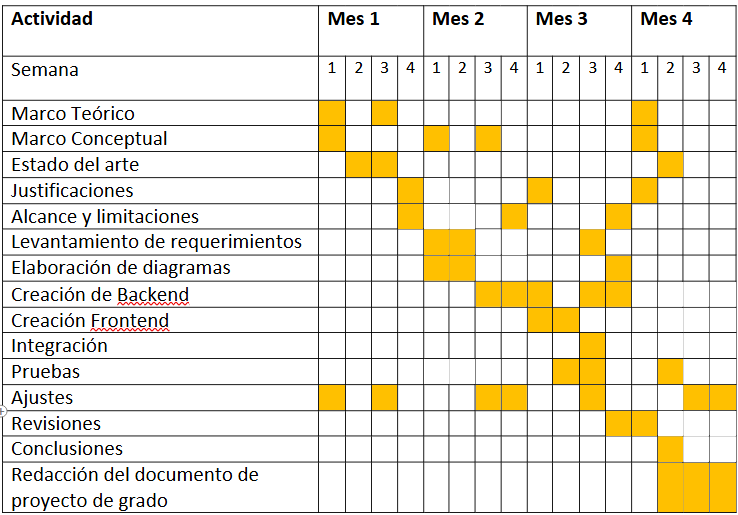
\includegraphics[width=\textwidth]{Images/Calendario.png}
%     \caption{Cronograma de Actividades del Proyecto.}
%     \label{fig:calendario}
% \end{figure}

% % Referencias
% \newpage
\printbibliography[
    heading=bibintoc,
    title={Referencias}
]
\end{document}
